\documentclass[12pt,leqno]{report}
%\usepackage{setspace}
%\singlespace
%\usepackage[protrusion=true, expansion=true]{microtype}
%\usepackage[protrusion=true]{microtype}

\sloppy

\usepackage{urcsbiblio,urcsthesis}
\usepackage{url}
\usepackage{latexsym}
\usepackage{amsmath}
%\usepackage{algpseudocode}
\usepackage{graphicx}
%\usepackage[dvips]{graphicx}
\usepackage{multirow}
\usepackage[utf8]{inputenc}
\usepackage[encapsulated]{CJK}
\usepackage{pst-all}
\usepackage{color}
\usepackage{psfrag}
%\usepackage{pst-qtree}
\usepackage{pstricks}
\usepackage{pstricks-add}
\usepackage{amsmath,bm}
\usepackage{array}
%\usepackage[ruled,vlined]{algorithm2e}
\usepackage{subcaption}
%\usepackage{picins}
%\usepackage{algorithm}
\usepackage{tikz}
\usetikzlibrary{positioning}
\usetikzlibrary{shapes, arrows}
\tikzset{
    events/.style={ellipse, draw, align=center},
}
\usepackage{caption}
\usepackage{subcaption}
\usepackage{multirow}
%\usepackage{pst-node,pst-tree,pst-coil,avm}
%\input{pst-qtree}
%\renewcommand{\algorithmicrequire}{\textbf{Input:}}
%\renewcommand{\algorithmicensure}{\textbf{Output:}}
%\setlength\titlebox{6.5cm}    % Expanding the titlebox
%\usepackage{pst-node,pst-tree,pst-coil,pst-qtree}
\usepackage{times}
\usepackage{rotating} % CTAN/macros/latex/contrib/supported/rotating

\usepackage{enumerate}
%\usepackage{mathpazo}
%\usepackage{pst-qtree}
\psset{levelsep=2.5em,treesep=0pt,treefit=tight}
\usepackage{amsmath,amssymb}
%\usepackage{picins}
\newcommand{\boxnum}[1]{{\setlength{\fboxsep}{1pt}\raisebox{1pt}
{\hspace{1pt}\fbox{\tiny{\ensuremath{#1}}}\hspace{1pt}}}}
\newcommand{\ind}[1]{\ensuremath{^{\kern-0.5pt\boxnum{#1}}}}

\def\de{\rightarrow}
\def\la{\langle}
\def\ra{\rangle}
\def\state#1{\underbar{\textit{#1}}}

% for inside/outside sets
\def\ins#1{\mathrm{in}({#1})}
\def\out#1{\overline{\mathrm{in}}({#1})}

\usepackage{algorithm}
\usepackage[noend]{algorithmic}
\usepackage{tikz}
\usetikzlibrary{shapes,arrows}
%\usepackage[noend]{algorithmic}
%\usepackage[noend]{algpseudocode}

%\usepackage{setspace}
%\singlespace
%\usepackage[protrusion=true, expansion=true]{microtype}
%\usepackage[protrusion=true]{microtype}

\newcommand{\bigO}{{\cal O}}
\newcommand{\G}{{\cal G}}
\newcommand{\T}{{\cal T}}
\newcommand{\sub}{{\mathrm{sub}}}
\newcommand{\upsub}{{\mathrm{\overline{sub}}}}
\newcommand{\downsub}{{\mathrm{\underline{sub}}}}

\newcommand{\dottededge}{\ncdiag[arm=0,angleA=-90,angleB=90,linestyle=dotted]}
\newcommand{\blankedge}{\ncdiag[arm=0,angleA=-90,angleB=90,linestyle=none]}
\newcommand{\arrowedge}{\ncdiag[arm=0,angleA=-90,angleB=90,arrows=->]}
\newcommand{\blueedge}{\ncdiag[arm=0,angleA=-90,angleB=90,linecolor=blue]}

\newcommand{\mycircle}{\hspace{4pt}\raisebox{4pt}{\circle{6}}}
\newcommand{\myblackcircle}{\hspace{4pt}\raisebox{4pt}{\circle*{6}}}
%\DeclareMathOperator*{\argmax}{argmax}
%\DeclareMathOperator*{\argmin}{argmin}

\newcommand{\argmax}{\operatornamewithlimits{argmax}}
\newcommand{\argmin}{\operatornamewithlimits{argmin}}
\providecommand{\abs}[1]{\lvert#1\rvert}
\providecommand{\norm}[1]{\lVert#1\rVert}

\newtheorem{theorem}{Theorem}
\newtheorem{lemma}[theorem]{Lemma}
\newtheorem{proposition}[theorem]{Proposition}
\newtheorem{corollary}[theorem]{Corollary}
\newtheorem{definition}{Definition}

% for inside/outside sets
\def\ins#1{\mathrm{in}({#1})}
\def\out#1{\overline{\mathrm{in}}({#1})}

\usepackage{rotating} % CTAN/macros/latex/contrib/supported/rotating

\definecolor{LemonChiffon}{rgb}{1.,0.98,0.8}
\definecolor{PaleGreen}   {rgb}{0.88,1,0.88}
\definecolor{Pink}        {rgb}{1.,0.75,0.8}
\definecolor{Thistle}     {rgb}{0.85,0.75,0.85}

\newenvironment{proof}[1][Proof]{\begin{trivlist}
\item[\hskip \labelsep {\bfseries #1}]}{\end{trivlist}}

\newcommand{\qed}{\nobreak \ifvmode \relax \else
      \ifdim\lastskip<1.5em \hskip-\lastskip
            \hskip1.5em plus0em minus0.5em \fi \nobreak
                  \vrule height0.75em width0.5em depth0.25em\fi}


%\usepackage{ucs}
%\usepackage[T1]{fontenc}


\newcommand{\cntext}[1]{\begin{CJK}{UTF8}{cyberbit}#1\end{CJK}}
%\newcommand{\cntext}[1]{\begin{CJK}{UTF8}{cyberbit} {\fontspec{STSong}#1} \end{CJK}}
\newcommand{\pycntext}[2]{\begin{tabular}{c}#1\\\cntext{#2}\end{tabular}}

%\usepackage{acl-hlt2011}


%\setlength\titlebox{6.5cm}    % Expanding the titlebox

%\def\namecite{\newcite}

\usepackage{xspace}
\newcommand{\goesto}{\ensuremath{\rightarrow}\xspace}



%\thesisproposal



\definecolor{rblue}{RGB}{0,70,127}
\definecolor{dyellow}{RGB}{255,221,0}
\definecolor{uorange}{RGB}{248,151,26}
\definecolor{coolgray}{RGB}{215,217,218}
\definecolor{darkgreen}{RGB}{88,123,124}
\definecolor{ured}{RGB}{239,51,34}

\psset{levelsep=2.5em,treesep=0pt,treefit=tight}
\psset{arrowscale=2}

%\newtheorem{theorem}{Theorem}

\pdfinfo{
/Title (MCMC algorithms applications in various NLP problems)
/Author (Xiaochang Peng)
/Keywords (Thesis proposal, semantic parsing, decipherment-based machine translation, distributed representation, neural machine translation, natural language processing)
}

%\thesisproposal
\begin{document}
\begin{CJK}{UTF8}{cyberbit}

\title{MCMC algorithms for various NLP applications}
\author{Xiaochang Peng}
\thesissupervisor{Professor Daniel Gildea}

%\date{July, 2012}

\maketitle

\thispagestyle{empty}
%\thispagestyle{plain}
%\newenvironment{dedication}
%{\cleardoublepage \thispagestyle{empty} \vspace*{\stretch{1}}
%  \begin{center} \em}
%  {\end{center} \vspace*{\stretch{3}} }

\begin{abstract}
Markov Chain Monte Carlo (MCMC) methods are a class of sampling algorithms which samples from a probability distribution based on constructing a Markov chain that has the desired distribution as its equilibrium distribution. The states of the chain after a number of steps can be used as samples of the desired distribution. 
MCMC algorithms are widely used for calculating numerical approximations in spaces of high dimensionality, for example in Bayesian statistics, computational physics, computational biology and natural language processing (NLP).


In this proposal, we explore some applications of MCMC algorithms to various NLP problems. First we apply MCMC algorithms to sample synchronous grammar rules, with applications of phrase-based machine translation and semantic parsing. We define a distribution over derivation trees which represent a sequence of synchronous grammar rules applied to derive a language pair. We also propose a joint model which uses MCMC algorithms to sample phrases in a sentence and uses phrase-level
skip-gram model to learn a distributed representation for each phrase. Finally, we apply MCMC algorithms to learning translation models for decipherment-based machine translation where only monolingual datasets for each language are available.
\end{abstract}

\tableofcontents
%\listoftables
%\listoffigures

\chapter{Introduction}
MCMC algorithms is useful in reducing the search space.


The rest of the paper is structured as follows. In Chapter 2, I will discuss the MCMC algorithms in general. Chapter 3-6 will separately introduce the application of MCMC algorithms to 
semantic parsing, decipherment-based machine translation, distributed representation learning and neural machine translation. In Chapter 7, I conclude the proposal paper.

\break

\chapter{MCMC algorithms}
\label{chap:MCMC}
In this chapter, I mainly go over MCMC algorithms and review some properties of MCMC.
\section{Introduction}
\section{MCMC}
\subsection{Convergence property}
A first order Markov chain is defined as a series of states (assignments) of random variables $z^{(1)},\cdots,z^{(M)}$ such that the following conditional independence property holds for $m \in {1,\cdots,M-1}$:
$$p({\bf z}^{(m+1)}|{\bf z}^{(1)}, \cdots, {\bf z}^{(m)})=p({\bf z}^{(m+1)}|{\bf z}^{(m)})$$
We define {\it transition probabilities} $T({\bf z}^{(m)},{\bf z}^{(m+1)})\equiv p({\bf z}^{(m+1)}|{\bf z}^{(m)})$. A ${\it homogeneous}$ Markov chain is one that
the transition probabilities are the same for all $m$.


The marginal probability for a state at the $m+1$-th position can be expressed in terms of the marginal probability for the previous state in the chain:
$$p({\bf z}^{(m+1)})=\sum_{p({\bf z}^{(m)})} T({\bf z}^{(m+1)}|{\bf z}^{(m)})p({\bf z}^{(m)})$$

A distribution is {\bf stationary} with respect to a Markov chain if each step in the chain leaves the distribution invariant. For a homogeneous Markov chain 
with transition probabilities $T(z',z)$, the distribution $p(z)$ is invariant if
$$p({\bf z}) = \sum_{{\bf z'}}T({\bf z'}, {\bf z})p({\bf z'})$$

One sufficient (but not necessary) condition for ensuring the required distribution $p(z)$ to be stationary is to choose the transition probabilities to satisfy the property
of {\it detailed balance}, defined by
$$T({\bf z}, {\bf z'})p({\bf z}) = T({\bf z'}, {\bf z})p({\bf z'})$$
With detailed balance satisfied, then the distribution is stationary:
$$\sum_{{\bf z'}}T({\bf z'}, {\bf z})p({\bf z'}) = \sum_{{\bf z'}}T({\bf z}, {\bf z'})p({\bf z}) = p({\bf z})$$

Our goal is to use Markov chains to sample from a given distribution. We can achieve this if we set up a Markov chain such that the desired distribution is invariant. However, we must also require that for $m \rightarrow \infty$, the distribution $p({\bf z}^{(m)})$ converges to the required invariant distribution $p({\bf z})$, irrespective of the choice of initial distribution $p({\bf z}^{(0)})$. This property is called {\it ergodicity}, and the stationary distribution is then called the {\it equilibrium} distribution.


A Markov chain is {\it irreducible} if for $\forall a, b\in \Pi$, $\Pi$ is the value space for ${\bf z}$, $\exists m\geq 0$, s.t. $p({\bf z}^{(m)}=b|{\bf z}^{(0)}=a)>0$. That is, any state in the value space can be reached within
finite numbers of steps from any starting state. An irreducible Markov chain is {\it aperiodic} if $\forall a \in \Phi$, {\it gcd}\{$m:p({\bf z}^{(m)}=a|{\bf z}^{(0)}=a)>0$\} = 1. Where {\it gcd} is the greatest common divisor of a series of numbers.
Based on these definitions, we can define the ergodic theorem.
\begin{theorem}
If $({\bf z}^{(0)},{\bf z}^{(1)},\cdots,{\bf z}^{(n)})$ is an irreducible (homogeneous) discrete Markov Chain with a stationary
distribution $p^{*}({\bf z})$, then: 
$$\frac{1}{n}\sum_{i=1}^{n}f({\bf z}^{(i)}) \xrightarrow[n\rightarrow \infty]{} Ef({\bf z})$$ 
where ${\bf z}~ p^{*}({\bf z})$,
for any bounded function $f:z\rightarrow \mathbb{R}$ 
If further, it is aperiodic, then $p({\bf z}^{(n)}|{\bf z}^{(0)})\xrightarrow[n\rightarrow \infty]{} p^{*}({\bf z})$
\end{theorem}
Ergodic theorem can be used to define Markov chains that regardless of which state we start from, the distribution of the states will converge to the equilibrium distribution after
a number of steps.

\section{Types of MCMC algorithms}
\subsection{Metropolis-Hastings algorithm}
The Metropolis-Hastings algorithm was first introduced by \namecite{hastings1970monte}, which applies to cases where the proposal distribution is not symmetric.
Assume the current hidden state at time $t$ to be ${\bf z^{(t)}}$, we then draw a sample ${\bf z^{*}}$ from the distribution $q({\bf z}| {\bf z^{(t)}})$ and accept it with the following probability:
$$A({\bf z^{*}}, {\bf z^{(t)}})= \min \Big(1, \frac{\tilde{p}({\bf z^{*}})q({\bf z^{(t)}}| {\bf z^{*}})}{\tilde{p}({\bf z^{(t)}})q({\bf z^{*}}| {\bf z^{(t)}})}\Big)$$
Evaluating the acceptance rate does not require knowledge about the normalization constant $Z_p$ in the distribution $p({\bf z})=\frac{\tilde{p}({\bf z})}{Z_p}$. $p({\bf z})$ is a stationary distribution with respect
to the Markov chain. We can verify it with proving detailed balance:
\begin{equation}
\begin{split}
    p({\bf z}) q({\bf z}|{\bf z'}) A({\bf z'}, {\bf z}) &= \min (p({\bf z})q({\bf z}|{\bf z'}),p({\bf z'})q({\bf z'}|{\bf z})) \\ &= \min (p({\bf z'})q({\bf z'}|{\bf z}), p({\bf z})q({\bf z}|{\bf z'})) \\ &= p({\bf z'}) q({\bf z'}|{\bf z}) A({\bf z}, {\bf z'})
\end{split}
\end{equation}
For Metropolis-Hastings algorithms the specific choice of proposal distribution has a great effect on the performance. For continuous variable spaces, a common choice is usually a Gaussian centered on
the current state. And the choice of variance parameter would balance between acceptance rate and the convergence speed.
\subsection{Gibbs Sampling}
Gibbs sampling~\cite{geman1984stochastic} is another widely used MCMC algorithm, which can be seen as a special case of the Metropolis-Hastings algorithm. 


Consider we wish to sample from the distribution $p({\bf z})=p(z_1,\cdots ,z_M)$ and we start from an initial state. Each step of the Gibbs sampling algorithm involves replacing the value of one of the variables 
by a value drawn from the distribution of that variable conditioned on the values of the remaining variables. In the $i$-th step we replace $z_i$ by a value drawn from the distribution $p(z_i|{\bf z_{\setminus i}})$, where $z_i$ denotes the $i$-th component of ${\bf z}$, 
and ${\bf z_{\setminus i}}$ denotes $z_1,\cdots,z_M$ but with $z_i$ omitted. This procedure is repeated either by cycling through the variables
in some particular order or by choosing the variable to be updated at each step at random from some distribution. In traditional NLP problems, the
hidden states ${\bf z}$ are usually structured as a sequence, a tree or a directed graph which usually provides explict order
for traversal and therefore for Gibbs update.
\begin{algorithm}[t]
\small
\caption{Gibbs Sampling}
\begin{algorithmic}[1]
\STATE{Initialize \{$z_i: i = 1, \cdots, M$\}}
\FOR{$\tau = 1,\cdots , T$:} 
\STATE{-Sample $z_1^{(\tau +1)}\sim p(z_1|z_2^{(\tau)},z_3^{(\tau)}, \cdots,z_M^{(\tau)})$} 
\STATE{-Sample $z_2^{(\tau +1)}\sim p(z_2|z_1^{(\tau+1)},z_3^{(\tau)}, \cdots,z_M^{(\tau)})$}
\STATE{$\vdots$}
\STATE{-Sample $z_j^{(\tau +1)}\sim p(z_j|z_1^{(\tau+1)},\cdots z_{j-1}^{(\tau+1)}, z_{j+1}^{(\tau)}\cdots,z_M^{(\tau)})$}
\STATE{$\vdots$}
\STATE{-Sample $z_M^{(\tau +1)}\sim p(z_M|z_1^{(\tau+1)},z_2^{(\tau+1)}, \cdots,z_{M-1}^{(\tau+1)})$}
\ENDFOR
\end{algorithmic}
\label{alg:gibbs}
\end{algorithm}
\section{Conclusion}
In this chapter, I have gone through some properties of MCMC algorithms that enable the Markov chain to converge to the desired distribution after
finite number of steps. Two widely used MCMC algorithms, Metropolis-Hastings and Gibbs Sampling algorithms, provide simple but power tools to sample from intractable probability distributions.

\break

%\chapter{AMR parsing}
%\label{chap:amr}
%In this chapter, we apply MCMC algorithm to learn synchronous graph grammars for mapping strings
to graphs structure. Specifically, we learn Synchronous Hyperedge Replacement Grammar (SHRG) rules from a forest that represents likely derivations consistent with a fixed string-to-graph 
alignment. We make an analogy of string-to-AMR parsing to the task of phrase-based machine translation and
come up with an efficient algorithm to learn graph grammars from string-graph pairs. We propose an effective
approximation strategy to resolve the complexity issue of graph compositions. We also show some useful strategies
to overcome existing problems in an SHRG-based parser and present preliminary results of a graph-grammar-based approach. 
%\section{Introduction} 
%Abstract Meaning Representation (AMR) \cite{banarescu2013abstract} is a semantic formalism where the meaning 
%of a sentence is encoded as a rooted, directed graph. 
%Figure~\ref{fig:amr-example} shows an example of the edge-labeled representation of an AMR 
%graph where the edges are labeled while the nodes are not. The label of the leaf edge going out of a node represents 
%the concept of the node, and the label of a non-leaf edge shows the relation between the concepts of the two nodes it connects to. 
%This formalism is based on propositional logic and neo-Davidsonian event representations~\cite{parsons1990events,Davidson:1967}.
%AMR does not encode quantifiers, tense and modality, but it jointly encodes a set of selected semantic phenomena which renders
%it useful in applications like question answering and semantics-based machine translation.
%
%\begin{figure}
%\begin{center}
%\scalebox{0.50}{
%    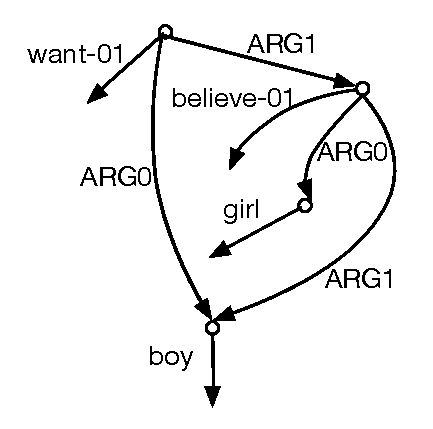
\includegraphics{./amr_example.eps}
%}
%\caption{An example of AMR graph representing the meaning of: ``The boy wants the girl to believe him"}
%\label{fig:amr-example}
%\vspace{-1em}
%\end{center}
%\end{figure}
%The task of AMR graph parsing 
%is to map natural language strings to AMR semantic graphs. \namecite{flanigan2014discriminative} propose a two-stage parsing
%algorithm which first maps meaningful continuous spans on the string side to concept fragments
%on the graph side, and then in the second stage adds additional edges to
%make all these fragments connected. Concept identification \cite{flanigan2014discriminative,pourdamghanialigning} can be considered as an important first step to
%relate components of the string to components in the graph.
%
%
%\namecite{wang-xue-pradhan:2015:NAACL-HLT} also present a two-stage procedure where they first use a dependency parser
%trained on a large corpus to generate a dependency tree for each sentence. In the second step, a transition-based algorithm
%is used to greedily modify the dependency tree into an AMR graph. The 
%benefit of starting with a dependency tree instead of the original sentence is that the dependency structure is 
%more linguistically similar to an AMR graph and provides more direct feature information within limited
%context.
%
%
%Hyperedge replacement grammar (HRG) is a context-free rewriting formalism for generating graphs~\cite{drewes+al:1997}. 
%Its synchronous counterpart, SHRG, can be used for transforming a graph from/to another structured representation such as a string
%or tree structure. HRG has great potential for applications in natural language understanding and generation,
%and also semantics-based machine translation. 
%
%
%Given a graph as input, finding its derivation of HRG rules is NP-complete~\cite{drewes+al:1997}. 
%\namecite{chiang-acl13} describe in detail a graph recognition algorithm
%and present an optimization scheme which enables the
%parsing algorithm to run in polynomial time when the treewidth and degree
%of the graph are bounded. However, there is still no real system available
%for parsing large graphs.
%
%
%An SHRG can be used for AMR graph parsing where each SHRG rule consists of a pair of a CFG rule and an HRG rule, 
%which can generate strings and AMR graphs in parallel. 
%\namecite{jones2012semantics} present a Syntactic Semantic Algorithm that learns SHRG by matching minimal parse constituents
%to aligned graph fragments and incrementally collapses them into hyperedge nonterminals. 
%The basic idea is to use the string-to-graph alignment and syntax information to constrain the possible HRGs.
%
%
%Learning SHRG rules 
%from fixed string-to-graph alignments is a similar problem to extracting machine translation rules from fixed word
%alignments, where we wish to automatically learn the best granularity for the rules with which to analyze each
%sentence. \namecite{chung-cl14} present an MCMC sampling schedule to learn Hiero-style SCFG rules \cite{ChiangCL} by sampling 
%tree fragments from phrase decomposition forests, which represent all possible
%rules that are consistent with a set of fixed word alignments, making use of the property that each SCFG rule in the 
%derivation is in essence the 
%decomposition of a larger phrase pair into smaller ones.
%
%
%In this paper, we make an analogy to treat fragments in the graph language as phrases in the natural language string 
%and SHRG rules as
%decompositions of larger substring, graph fragment pairs into smaller ones. 
%Graph language is different
%from string language in that there is no explicit order to compose the graph and there is an exponential number of possible 
%compositions. We propose a strategy that uses the left-to-right order of the string to constrain the structure of the 
%derivation forest and experiment with different tactics in dealing with unaligned words on the string side and unaligned
%edges on the graph side.
%
%
%\section{Hyperedge Replacement Grammar}
%\begin{figure}
%\begin{center}
%\resizebox{\linewidth}{!}{
%\scalebox{0.45}{
%    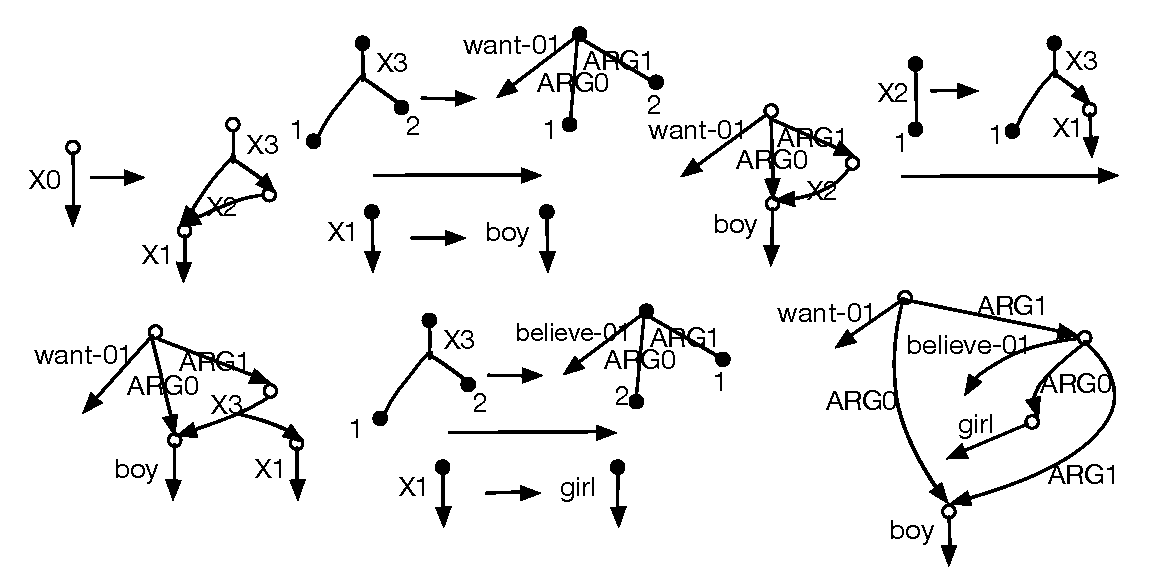
\includegraphics{./HRG.eps}
%}
%}
%\caption{The series of HRG rules applied to derive the AMR graph of ``The boy wants the girl to believe him". The first rule is directly shown. The other HRG rules
%are either above or below each right arrow. The white circle shows the root of each hyperedge. The indexes in each rule show the one-to-one mapping
%between the attachment nodes of l.h.s.\ nonterminal edges and the external nodes of the r.h.s.\ subgraph}
%\label{fig:hrg-example}
%\vspace{-1em}
%\end{center}
%\end{figure}
%Hyperedge replacement grammar (HRG) is a context-free rewriting formalism for graph generation \cite{drewes+al:1997}. 
%HRG is like CFG in that it rewrites nonterminals independently.
%While CFG generates natural language strings by successively rewriting nonterminal tokens, the nonterminals in 
%HRG are hyperedges, and each rewriting step in HRG replaces a hyperedge nonterminal with a subgraph instead of a span of a string.
%\subsection{Definitions}
%In this paper we only use edge-labeled graphs
%because using both node and edge labels complicates the definitions in our HRG-based approach. Figure~\ref{fig:hrg-example} 
%shows a series of HRG rules applied to derive the AMR graph shown in Figure~\ref{fig:amr-example}.
%
%
%We start with the definition of hypergraphs. An {\em edge-labeled, directed hypergraph} is a tuple $H=\langle V,E,l,X\rangle$, where $V$ is a finite set of nodes, $E\subseteq V^+$ is
%a finite set of hyperedges, each of which will connect to one or more nodes in $V$. $l: E\to L$ defines a mapping from each 
%hyperedge to its label from a finite set $L$. Each hyperedge is an atomic item with an ordered list of nodes it connects to, which 
%are called attachment nodes. The {\em type} of a hyperedge
%is defined as the number of its attachment nodes.  $X\in V^*$ defines an ordered list of distinct nodes called
%{\em external nodes}. 
%The ordered external nodes specify how to fuse a
%hypergraph with another graph, as we will see below.
%In this paper, we alternately use the terms of 
%hypergraph and graph, hyperedge and edge, and also phrase, substring and span for brevity.
%
%
%An HRG is a rewriting formalism $G=\langle N,T,P,S \rangle$, where $N$ and $T$ define two disjoint finite sets called nonterminals 
%and terminals. $S\in N$ is a special nonterminal
%called the start symbol. $P$ is a finite set of productions of the form $A\to R$, where $A\in N$ and $R$ is a 
%hypergraph with edge labels over $N\cup T$ and with nonempty external nodes $X_R$. We have the constraint that the type of the
%hyperedge with label $A$ should coincide with the number of nodes in $X_R$. In our grammar, each nonterminal
%has the form of $Xn$, where $n$ indicates the type of the hyperedge. Our special start symbol is separately denoted as $X0$.
%
%
%The rewriting mechanism replaces a nonterminal 
%hyperedge with the graph fragment specified by a production's
%righthand side (r.h.s),\ attaching each external node of the 
%r.h.s.\ to the corresponding attachment node of the lefthand side.
%Take Figure~\ref{fig:hrg-example} as an example. 
%Starting from our initial hypergraph with one edge 
%labeled with the start symbol $``X0"$, we select one edge with nonterminal label in our current hypergraph, 
%and rewrite it using a rule in our HRG\@. The first rule rewrites
%the start symbol with a subgraph shown on the r.h.s..\ We continue the rewriting steps 
%until there are no more nonterminal-labeled edges. 
%
%
%The synchronous counterpart of HRG can be used for transforming graphs from/to another form of natural language representation. 
%Productions have the form $(A\to \langle S, R\rangle , \sim)$, where $A \in N$ and $S$ and $R$ are called the source and the target and at least one of them should be
%hypergraphs over $N\cup T$. $\sim$ is a bijection linking nonterminals mentions in $S$ and $R$.
%In our case, the source side is a CFG and the target side is an HRG\@. Given such a synchronous grammar and a string as input, we can 
%parse the string with the CFG side and then derive the counterpart graph by deduction from the derivation. The benefit of 
%parsing with SHRG is that the complexity is bounded by a CFG-like parsing.
%
%\subsection{SHRG-based AMR graph parsing}
%\begin{figure}
%\begin{center}
%\resizebox{\linewidth}{!}{
%\scalebox{0.45}{
%    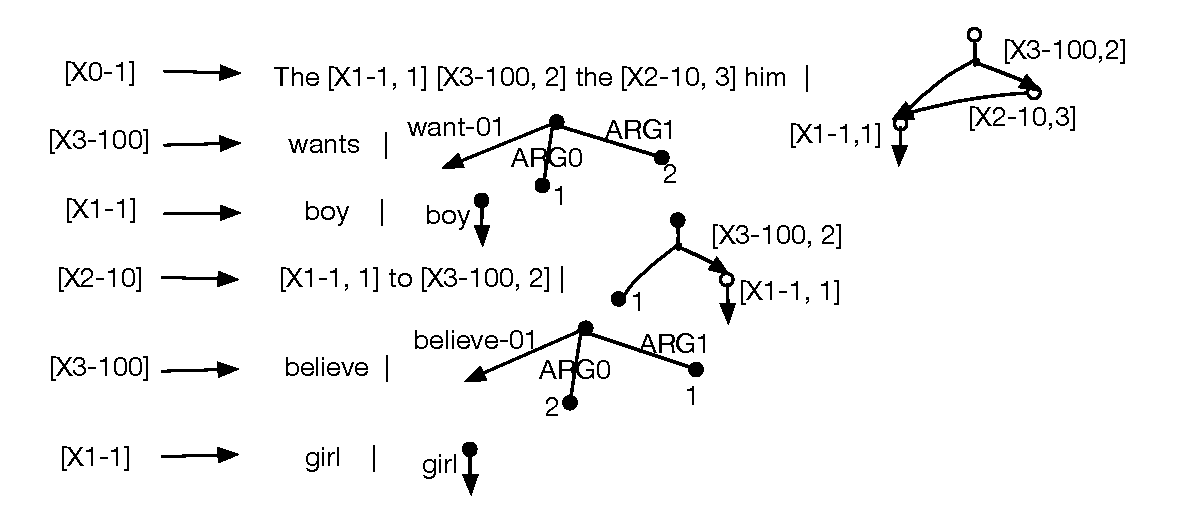
\includegraphics{./SHRGrules.eps}
%}
%}
%\caption{A series of symbol-refined SHRG rules used to derive the AMR graph for the sentence ``The boy wants the girl to believe him".}
%\label{fig:shrg-example}
%\vspace{-1em}
%\end{center}
%\end{figure}
%We write down AMR graphs as rooted, directed, edge-labeled graphs. There is exactly one leaf edge 
%going out of each node, the label of which represents the concept of the node. We define
%this leaf edge as {\bf concept edge}. In Figure~\ref{fig:amr-example}, for example, the edge labeled 
%with ``boy", ``want-01", ``girl" or ``believe-01" connects to only one node in the AMR graph and
%each label represents the concept of that node.
%AMR concepts are either English words (``boy"), PropBank framesets (``want-01"), or special keywords like
%special entity types, quantities, and logical conjunctions. The label of each non-leaf edge shows the relation
%between the AMR concepts of the two nodes it connects to. %In the rest of the paper we will use ``want" and ``believe" instead of they frameset representation for brevity.
%
%
%The constraint of having exactly one concept edge for each node 
%is not guaranteed in general SHRG\@. Our strategy for maintaining the AMR graph structure is to refine the 
%edge nonterminal label with an extra binary
%flag, representing whether it will have a concept edge in the
%final rewriting result, for each external node. The basic intuition is to explicitly enforce the one concept edge constraint
%in each nonterminal so that no additional concept edge is introduced after applying each rule. The graph
%derived from this type of SHRG is guaranteed to have exactly one concept edge at each node.
%
%
%Figure~\ref{fig:shrg-example} shows one example of our symbol-refined SHRG\@.
%For each nonterminal $Xi$-$b_1\cdots b_i$, $i$ defines the type of the nonterminal, while
%each $b_i$ indicates whether the $i$-th external node will have a concept edge
%in the rewriting result.\footnote{$X0$-1 is different as $X0$ is the start symbol of type one and should always have a concept edge at the root}
%%For each $[Xi$-$b_1\cdots b_i, j]$, $i$ defines the type of the nonterminal, while
%%each $b_i$ indicates whether the $i$-th external node will have a concept edge
%%in the rewriting result.\footnote{$X0$-1 is different as $X0$ is the start symbol of type one and should always have a concept edge at the root} 
%%$j$ indicates the one to one mapping from the nonterminals
%%on the string side to the nonterminal edges on the graph side.
%The second rule, for example, rewrites nonterminal $X3$-100 with {\em wants} on the string side and a hypergraph with three external nodes where 
%the root has a concept edge {\em :want-01} as the first binary flag 1 indicates, while the other two external nodes do not with the binary flag 0. 
%This guarantees that when we integrate the r.h.s.\ into
%another graph, it will introduce the concept edge {\em :want-01} to the first fusing position
%and no concept edge to the next two.
%
%
%While this refinement might result in an exponential number of nonterminals with respect to the maximum type of hyperedges, 
%we found in our experiment that most of the nonterminals
%do not appear in our grammar. We use a maximum edge type of 5, which also results in a relatively small nonterminal set.
%\section{Sampling SHRG from forests}
%The fragment decomposition forest provides a compact representation of all possible SHRG rules that are consistent with a fixed string-to-graph 
%alignment. Each SHRG rule in the derivation is in essence the decomposition of 
%larger phrase, graph fragment pairs on the left hand side (l.h.s.)\ into smaller ones on the r.h.s.\ and is
%encoded in a tree fragment in the forest. Our goal is to learn an SHRG from this forest.
%We first build a forest representation of possible derivations and then use an MCMC algorithm to
%sample tree fragments from this forest representing each rule in the derivation.
%\subsection{Fragment Decomposition Forest}
%We first proceed to define the {\bf fragment decomposition forest}. The fragment decomposition forest is a variation of
%the phrase decomposition forest defined by \namecite{chung-cl14} where the target side is a graph instead of a string.
%
%
%$$\resizebox{.88\hsize}{!}{$\displaystyle
%\overbrace{The}^\text{$\emptyset$}\ \overbrace{boy}^\text{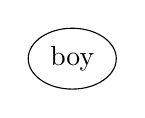
\begin{tikzpicture}\draw (0,0) node[draw,ellipse]{boy}; \end{tikzpicture}}
%\overbrace{wants}^\text{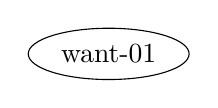
\begin{tikzpicture}\draw (0,0) node[draw,ellipse]{want-01};  \end{tikzpicture}} %{want-01};
%\overbrace{the}^\text{$\emptyset$}
%\overbrace{girl}^\text{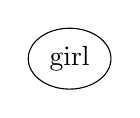
\begin{tikzpicture}\draw (0,0) node[draw,ellipse]{girl}; \end{tikzpicture}}
%\overbrace{to}^\text{$\emptyset$}
%\overbrace{believe}^\text{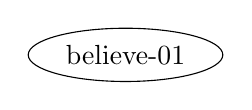
\begin{tikzpicture}\draw (0,0) node[draw,ellipse]{believe-01}; \end{tikzpicture}}
%\overbrace{him}^\text{$\emptyset$}$}
%$$
%A {\bf phrase} $p=[i, j]$ is a set of continuous word indices $\{i,i+1,\ldots ,j-1\}$. A {\bf fragment} $f$ is 
%a hypergraph with external nodes $X_f$. A string-to-graph alignment $h: P \to F$ defines the mapping from
%spans in the sentence to fragments in the graph.
%Our smallest phrase-fragment pairs are the string-to-graph alignments extracted using heuristic
%rules from \namecite{flanigan2014discriminative}.
%The figure above shows an example of the alignments for the sentence ``The boy wants the
%girl to believe him". The symbol $\emptyset$ represents that the word is not aligned to any concept in the AMR graph and this word is called an {\bf unaligned word}. 
%After this alignment, there are also left-over edges that are not aligned from any substrings, which are called
%{\bf unaligned edges}.
%
%
%Given an aligned string, AMR graph pair, 
%a phrase-fragment pair $n$ is a pair $([i, j], f )$ which defines a pair of a phrase $[i,j]$ and a fragment $f$ such
%that words in positions $[i,j]$ are only aligned to concepts in the fragment $f$ and vice versa (with unaligned words and edges omitted).
%%, the definition of which will be clear later
%A fragment forest $H=\langle V, E \rangle$ is a hypergraph made of a set of
%hypernodes $V$ and hyperedges $E$. Each node $n=([i, j], f)$ is {\bf tight} on the string side similar to 
%the definition by \namecite{Koehn-naacl03}, i.e., $n$ contains no unaligned words at its boundaries. 
%Note here we do not have the constraint that $f$ should be connected or single rooted, but we 
%will deal with these constraints separately in the sampling procedure.
%
%
% We define two phrases $[i_1,j_1],[i_2,j_2]$ to be \textit{adjacent} if word indices $\{j_1,j_1+1,\ldots ,
% i_2-1\}$ are all unaligned. We also define two fragments $f_1=\langle V_1, E_1 \rangle, f_2=\langle V_2, E_2\rangle$ to be \textit{disjoint}
%if $E_1 \cap E_2 = \emptyset$. And $f_1$ and $f_2$ are
%adjacent if they are disjoint and $f = \langle V_1 \cup V_2, E_1 \cup E_2\rangle$ is connected.
%We also define the $compose$ operation of two nodes: it takes
%%$n = ([i_1, j_2], f)$ to be the result of $compose$ operation of 
%two nodes $n_1=([i_1, j_1], f_1)$ and $n_2=([i_2, j_2], f_2)$ ($j_1 \leq i_2$) as input, and computes $f = \langle V_1 \cup V_2, E_1 \cup E_2\rangle$,
%the output is a composed node $n=([i_1, j_2], f)$. We say $n_1$ and $n_2$ are \textit{immediately adjacent} if $f$ is connected and single-rooted.
%
%
%\begin{figure}
%\begin{center}
%%\resizebox{\linewidth}{!}{
%\scalebox{0.30}{
%    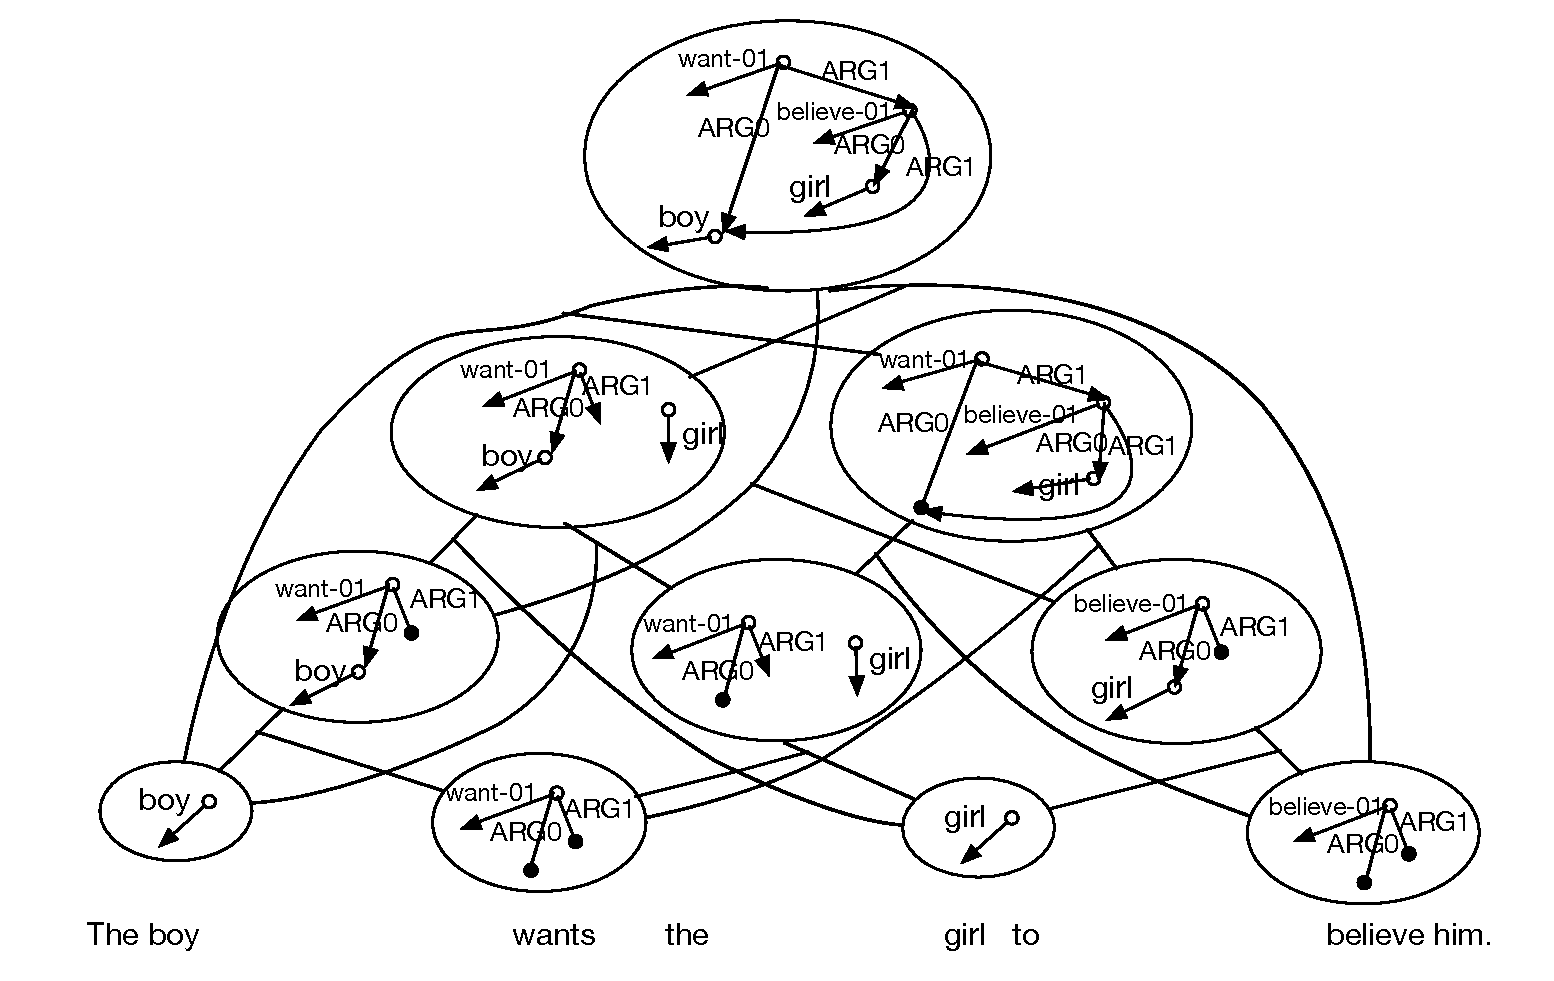
\includegraphics{./HRGForest.eps}
%}
%%}
%\caption{The fragment decomposition forest for the (sentence, AMR graph) pair for ``The boy wants the girl to believe him"}
%\label{fig:decompose-example}
%\vspace{-1em}
%\end{center}
%\end{figure}
%We keep composing larger phrase-fragment pairs (each one kept in a node of the forest) from smaller ones until we reach the root of the forest whose
%phrase side is the whole sentence and the fragment side is the complete AMR graph.
%We define {\bf fragment decomposition forest} to be made of all possible phrase-fragments pairs that can
%be decomposed from the sentence AMR graph pair. The fragment decomposition forest has the important property
%that any SHRG rule consistent with the string-to-graph alignment corresponds to a continuous
%tree fragment of a complete tree found in the forest. 
%
%
%While we can compose larger 
%phrases from smaller ones from left to right, there is no explicit order of composing the graph fragments. Also, the number of possible 
%graph fragments is highly exponential as we need to make a binary decision to decide each boundary node of the fragment and 
%also choose the edges going out of each boundary node of the fragment, unlike the polynomial numbers of phrases for fixed string alignment.
%
%
%Our bottom-up construction procedure starts from the 
%%string-to-graph alignment extracted using \namecite{flanigan2014discriminative}, which are our 
%smallest phrase-fragment pairs.
%We first index these smallest phrase-fragment pairs $([i_k, j_k], f_k), k = 1, 2, \ldots, n$ based on ascending order of their start positions 
%on the string side, i.e., 
%$j_k \leq i_{k+1}$ for $k = 1, 2, \ldots, n-1$. Even with this left-to-right order constraint from the string side, the complexity of
%building the forest is still exponential due to the 
%possible choices in attaching graphs edges that are not aligned to the string. 
%Our strategy
%is to deterministically attach each unaligned relation edge to one of the identified concept 
%fragments it connects to. We attach {\em ARG}s and {\em op}s to its head
%node and each other types of unaligned relations to its tail node.\footnote{Our intuition is that the ARG types for verbs and ops structure
%usually go with the concept of the head node. We assume that other relations are additional introduced to the head node, which resembles
%a simple binarization step for other relations.}
%
%\begin{algorithm}[t]
%\small
%\caption{A CYK-like algorithm for building a fragment decomposition forest}
%\begin{algorithmic}[1]
%    \STATE{For each smallest phrase-fragment pairs $([i_k, j_k], f_k)$, $k$ = $1, 2, \ldots , n$, attach unaligned edges to fragment $f_k$, denoting the result as $f_k'$. Build a node 
%    for $([i_k, j_k], f_k')$ and add it to chart item $c[k][k+1]$.} \label{1st}
%    \STATE{Extract all the remaining unaligned fragments, build a special unaligned node for each of them and add it to unaligned node set $unaligned\_nodes$} \label{2nd}
%    \STATE{Keep composing unaligned nodes with nodes in different chart items if they are immediate adjacent and add it to the same chart item} \label{3rd}
%    \FOR{$span$ from 2 to $n$} \label{4th}
%        \FOR{$i$ from 1 to $n$-$span$+1}
%            \STATE{$j$ = $i$ + $span$}
%            \FOR{$k$ from $i+1$ to $j-1$}
%                \FOR{$n1=([start_1, end_1], f_1)$ in $c[i][k]$}
%                    \FOR{$n2=([start_2, end_2], f_2)$ in $c[k][j]$}
%                        \IF{$f_1$ and $f_2$ are disjoint}
%                        \STATE{$new\_node$ = $compose(n1, n2)$} \label{new}
%                            \STATE{add incoming edge $(n1, n2)$ to $new\_node$}
%                            \IF{$n_1$ and $n_2$ are not {\em immediate adjacent}} \label{5th}
%                                \STATE{$new\_node.nosample\_cut$=True}
%                                \ENDIF \label{6th}
%                                \STATE{{\em insert\_node}($new\_node$, $c[i][j]$)} \label{7th}
%                        \ENDIF
%                    \ENDFOR
%                \ENDFOR
%            \ENDFOR
%        \ENDFOR
%    \ENDFOR
%  \end{algorithmic} 
%  \label{alg:forest} 
%\end{algorithm}
%Algorithm~\ref{alg:forest} shows our CYK-like forest construction algorithm. We maintain the length 1 chart items according to the order of each smallest phrase-fragment
%pair instead of its position in the string.\footnote{We use this strategy mainly because the alignments available do not have
%overlapping alignments, while our algorithm could still be easily adapted to a version that maintains the chart items with string
%positions when overlapping alignments are available} In line~\ref{1st}, we first attach unaligned edges to the smallest phrase-fragment pairs as stated before.
%After this procedure, we build a node for the $k$-th phrase-fragment (with unaligned edges added) pair and add it to chart item $c[k][k+1]$.
%Note here that we still have remaining unaligned edges; in line~\ref{2nd} we attach all unaligned edges going out from the same node as a single fragment and build a special 
%{\bf unaligned node} with empty phrase side and add it to $unaligned\_nodes$ set. In line~\ref{3rd}, we try to compose each unaligned node with one of the nodes in the length 1 chart items
%$c[k][k+1]$. If they are immediately adjacent, we add the composed node to $c[k][k+1]$. 
%The algorithm then composes smaller phrase-fragment pairs into larger ones (line~\ref{4th}). When we have composed two nodes $n_1, n_2$, we need to keep track of this
%incoming edge. We have the constraint in our grammar that the r.h.s.\ hypergraph of each rule
%should be connected and single rooted.\footnote{We should be able to get rid of both constraints as we are parsing on the string side.} Lines~\ref{5th} to ~\ref{6th} enforce this constraint
%by marking this node with a $nosample\_cut$ flag, which we will use in the MCMC sampling stage.
%The $insert\_node$ function will check if the node already exists in the chart item. If it already exists, then we only update the incoming edges for that node. Otherwise 
%we will add it to the chart item. 
%
%
%For some sentence-AMR pairs where there are too many nodes with unaligned edges going out, considering all possible compositions would result in
%huge complexity overhead. One solution we have adopted is to disallow disconnected graph fragments and do not add them to the chart items (Line~\ref{7th}). In practice, this pruning 
%procedure does not affect much of the final performance in our current setting.
%Figure~\ref{fig:decompose-example} shows the procedure of building the fragment decomposition forest 
%for the sentence ``The boy wants the girl to believe him".
%\subsection{MCMC sampling}
%Sampling methods have been used to learn Tree Substitution Grammar (TSG) rules from derivation trees \cite{cohn-2009-inducing,PostGildea-acl09} for TSG learning. 
%The basic intuition is to automatically learn the best granularity for the rules
%with which to analyze our data. Our problem, however, is different in that we need to
%sample rules from a compact forest representation. We need to sample one tree from the forest, and then
%sample one derivation from this tree structure, where each tree fragment represents one rule in the derivation. Sampling tree fragments from forests is described in detail in \namecite{chung-cl14} and \namecite{peng-gildea-emnlp14}.
%
%
%We formulate
%the rule sampling procedure with two types of variables: an edge variable $e_n$ representing which incoming hyperedge is chosen at a given node $n$ in the 
%forest (allowing us to sample one tree from a forest) and a cut variable $z_n$ representing whether node $n$ in forest is a boundary between two SHRG rules
%or is internal to an SHRG rule (allowing us to sample rules from a tree). 
%Figure~\ref{fig:sampled-example} shows one sampled derivation from the forest.
%We have sampled one tree from the forest using the edge variables.  We also have a 0-1 variable at each node in this tree where 0 represents the 
%current node is internal to an SHRG rule, while 1 represents the current node is the boundary of two SHRG rules.
%\begin{figure}
%\begin{center}
%%\resizebox{\linewidth}{!}{
%\scalebox{0.30}{
%    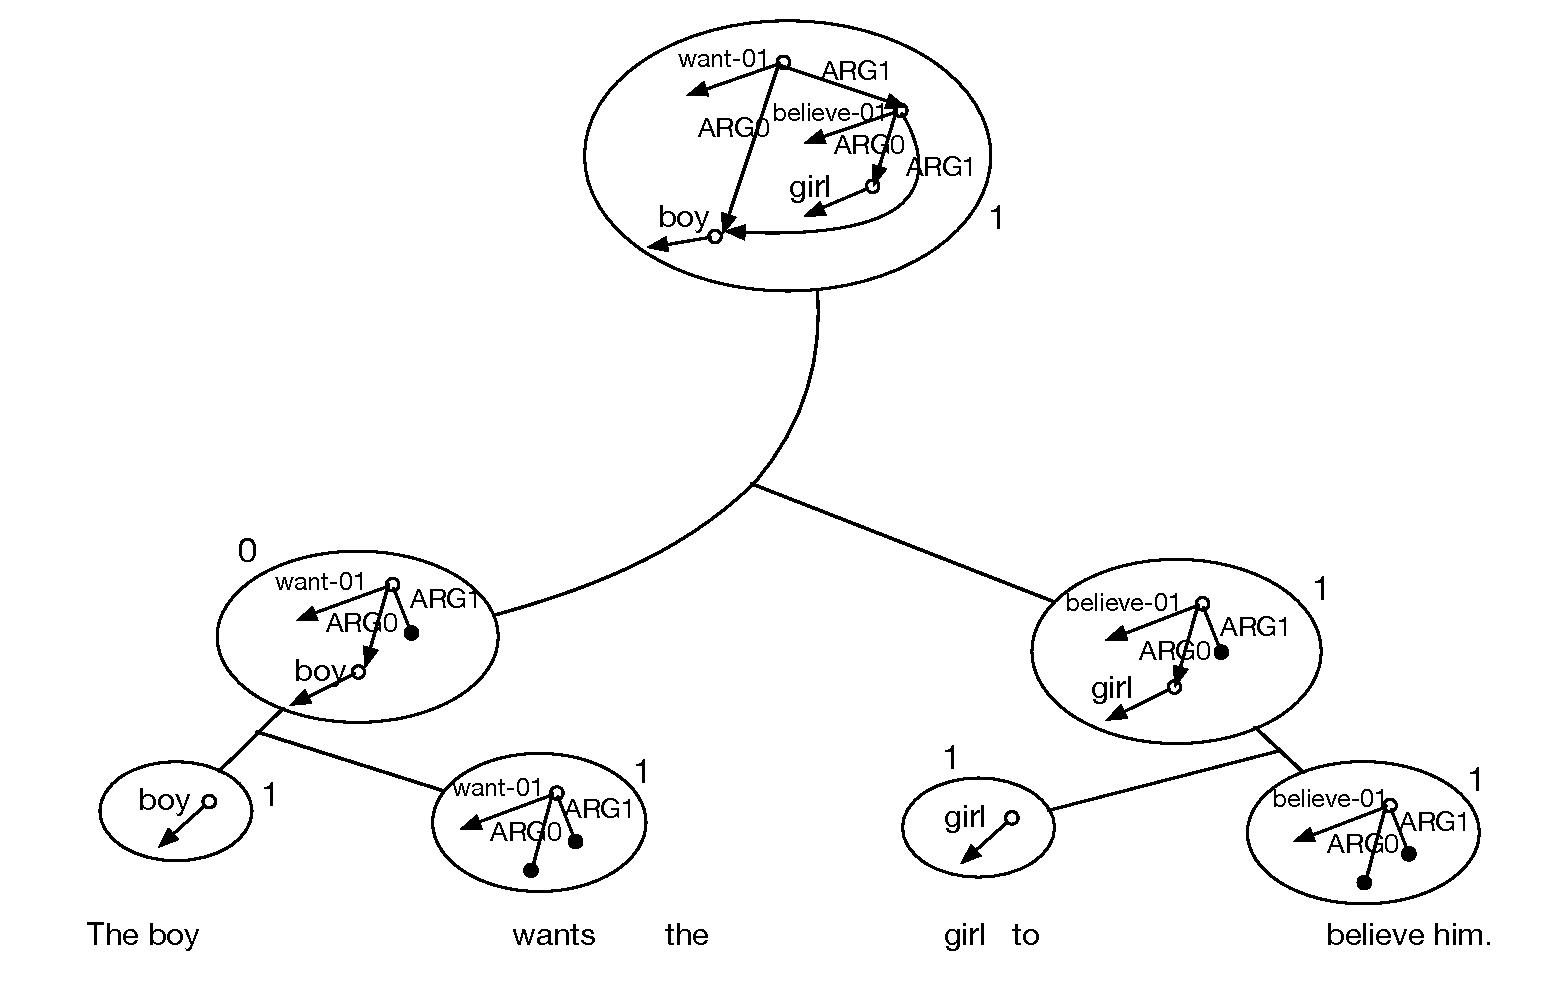
\includegraphics{./Sampled.eps}
%}
%%}
%\caption{The sampled derivation for the (sentence, AMR graph) pair for ``The boy wants the girl to believe him"}
%\label{fig:sampled-example}
%\end{center}
%\end{figure}
%
%Let all the edge variables form the random vector $Y$ and all the cut variables form the random vector $Z$. Given an assignment $y$ to the edge variables and assignment $z$ to the cut variables, our desired distribution is proportional to the product of weights of the rules specified by the assignment:
%\begin{equation}\label{eq:tsg}
% P_t(Y=y, Z=z) \propto \prod_{r \in \tau(y, z)} w(r) 
%\end{equation}
%where $\tau(y, z)$ is the set of rules identified by the assignment and $w(r)$ is the weight for each individual rule. We use a generative model based on a Dirichlet Process (DP) defined over composed rules. We draw a distribution $G$ over rules from a DP, and then rules from $G$. 
%\begin{align*}
%G\mid \alpha,P_0\sim& Dir(\alpha,P_0)\\
%r\mid G\sim& G
%\end{align*}
%
%We define two rules to have the same {\bf rule type} if they have the same string and hypergraph
%representation (including order of external nodes) on the r.h.s..%\footnote{We use special technique of hashing the edge labels, depth of nodes and external nodes sequence to decide the type of graph}
%For the base distribution $P_0$, we use a uniform distribution where all rules of the same size have equal probability.
%By marginalizing out $G$ we get a simple posterior distribution over rules which can be derived using the Chinese Restaurant Process (CRP). 
%
%
%We define a 
%table of counts $N=\{N_C\}_{C\in I}$ which memorizes different categories of counts in 
%the previous assignments, where $I$
%is an index set for different categories of counts. Each $N_C$ is a vector of counts for category $C$. 
%We have the following probability over rule $r$ given the previous count table $N$:
%\begin{equation}
%P(r_i = r| N) = \frac{N_R(r) + \alpha P_0 (r)}{n + \alpha }
%\end{equation}
%here in the case of DP, $I=\{R\}$, where $R$ is the index for the category of rule counts.%\footnote{Using this denotation, we can also adopt other priors like Pitman-Yor or other process priors as long as they satisfy exchangeability property} $N_R(r)$ is the number of times that rule $r$ has been observed in the previous assignment, $n=\sum_r N_R(r)$ is the total number of rules observed.
%
%We use the {\em top-down} sampling algorithm of \namecite{chung-cl14} which samples cut and edge variables from top down and one at a time.
%% (see Algorithm~\ref{alg:topdown}). 
%For each node $n$, we denote the composed rule type
%that we get when we set the cut of node $n$ to 0 as $r_1$ and the two 
%split rule types that we get when we set the cut to 1 as $r_2, r_3$. We sample the cut value $z_i$ of the 
%current node according to the posterior probability:
%\begin{equation}
%\label{eq:cut}
%%$$
%\resizebox{.88\hsize}{!}{$\displaystyle
%P(z_i = z| N) = 
%\begin{cases} 
%\frac{ P (r_1| N) }{P (r_1|N) + P (r_2| N) P (r_3| N') } &\mbox{if } z = 0 \\ 
%\frac{ P (r_2| N) P (r_3| N') }{P (r_1| N)+ P (r_2| N) P (r_3| N') } &\mbox{otherwise}
%\end{cases}$}
%%$$
%\end{equation}
%where the posterior probability $P(r_i|N)$ is according to a DP, 
%and $N, N'$ are tables of 
%counts. In the case of DP, $N, N'$ differ only in the rule counts of $r_2$, where $N'_R(r_2)= 
%N_R(r_2)+1$.
%
%
%As for edge variables $e_i$, we refer to the set of composed rules turned on below $n$ including the 
%composed rule fragments having $n$ as an internal or root node as $\{r_1,\ldots,r_m\}$. We have the 
%following posterior probability over the edge variable $e_i$:
%\begin{equation}
%\resizebox{.88\hsize}{!}{$\displaystyle
%P(e_i = e| N) \propto \prod_{i=1}^m P(r_i| N^{i-1}) \prod_{v \in \tau(e)\cap \mbox{in}(n)} \mbox{deg}(v)
%$}
%\end{equation}
%where $\mbox{deg}(v)$ is the number of incoming edges for node $v$, 
%$\mbox{in}(n)$ is the set of nodes 
%in all subtrees under $n$, and $\tau(e)$ is the tree specified when we set $e_i = e$. $N^0$ to $N^m$ 
%are tables of counts where $N^0 = N$, $N^i_R(r_i) = N^{i-1}_R(r_i) + 1$ in the case of DP.
%
%
%After we have sampled one SHRG derivation from the forest, we still need to keep track of the place where each nonterminal edge attaches.
%As we have maintained the graph fragment it represents in each node of the forest, we can retrieve the attachment nodes of each hyperedge in the r.h.s.\ by tracing at 
%which graph nodes two fragments fuse with each other. We perform this rule extraction procedure from top-down and maintain the order of attachment nodes of each r.h.s.\
%nonterminal edge.
%When we further rewrite a nonterminal edge, we need to make sure that it keeps the order of the attachment nodes in its parent rule. 
%As for the unaligned words, we just insert all the omitted unaligned words in the
%composition procedure. We also add additional rules including the surrounding 2 unaligned words context to
%make sure there are terminals on the string side.
%
%\subsection{Phrase-to-Graph-Fragment Alignment Extraction}
%Aside from the rules sampled using the MCMC algorithm,
%we also extract a phrase-to-graph-fragment alignment table from the fragment decomposition forest.
%This step can be considered as a mapping of larger phrases made of multiple identified spans (plus unaligned words) to a larger fragments made of multiple concept fragments (plus the way they connect using unaligned edges).
%
%
%Our extraction happens along with the forest construction procedure. In line~\ref{1st} of Algorithm~\ref{alg:forest}
%we extract one rule for each smallest phrase-fragment pairs before and after the unaligned
%edges are attached. We also extract one rule for each newly constructed node after line~\ref{new} 
%if the fragment side of the node is single-rooted.\footnote{Here we will also look at the surrounding 2 unaligned words to fix partial alignment and noise introduced
%by meaningful unaligned words}
%We do not extract rules after line~\ref{2nd} because it
%usually introduces additional noise of meaningful concepts which are unrecognized in the concepts
%identification stage. %For named entities and time expressions that can not be found in
%%our training data, we use the alignment result from the concept identification stage of \namecite{flanigan2014discriminative}.
%\section{Decoding}
%\subsection{Concept identification}
%During the decoding stage, first we need to identify meaningful spans in the sentence and map them to graph fragments on the graph side. Then we use SHRG rules to
%parse each sentence from bottom up and left to right, which is similar to constituent parsing. The recall of the concept identification stage from \namecite{flanigan2014discriminative} is 0.79, which means 21\% of the meaningful concepts are already lost at the beginning of the next stage. 
%
%
%Our strategy is to use lemma and POS tags information after the concept identification stage, we use it to recall some meaningful
%concepts. We find that, except for some special function words, most nouns, verbs and, adjectives
%should be aligned. We use the lemma information to retrieve unaligned words whose morphological form does not appear in our training data. 
%We also use POS tag information to deal with nouns and quantities. Motivated by the fact that AMR makes extensive use of PropBank framesets,
%we look up the argument structure of the verbs from the PropBank. Although the complicated abstraction of AMR
%makes it hard to get the correct concept for each word, the more complete structure can reduce the propagation of errors along the derivation tree.
%
%
%\subsection{AMR graph parsing}\label{sec:decode}
%We use Earley algorithm with cube-pruning \cite{ChiangCL} for the string-to-AMR parsing. 
%For each synchronous rule with $N$ nonterminals on its l.h.s., we build an $N+1$ dimensional cube and generate top $K$ candidates. 
%Out of all the hypotheses generated by all satisfied rules within each span $(i,j)$,we keep at most $K$ candidates for this span.
%Our glue rules will create a pseudo $R/ROOT$ concept and use $ARG$s relations to connect
%disconnected components to make a connected graph.
%%We use glue rule to connect two sub-graphs which a NULL edge.
%
%
%We use the following local features:
%\begin{enumerate}\footnotesize
%    \item StringToGraphProbability: the probability of a hypergraph given the input string
%    \item RuleCount: number of rules used to compose the AMR graph
%    \item RuleEdgeCount: the number of edges in the r.h.s.\ hypergraph 
%    \item EdgeType: the type of the l.h.s.\ nonterminal. For rules with same source side tokens, we prefer rules with smaller edge types.
%    \item AllNonTerminalPunish: one for rules which only have non-terminals on the source side.
%    \item GlueCount: one for glue rules.  
%\end{enumerate}
%As our forest structure is highly binarized, it is hard to capture the \textit{:op}n structure when $n$ is large because we limit the number
%of external nodes to 5. The most common \textit{:op} structure in the AMR annotation is the coordinate structure of items separated by ``;" or separated by ``," along with
%$and$. We add the following two rules:
%\begin{align*}
%    &\resizebox{.8\hsize}{!}{$[X\text{1-1}] -> [X\text{1-1}, 1] ; [X\text{1-1}, 2] ; \cdots ; [X\text{1-1}, n]\ |$}\\
%    &\quad \resizebox{.85\hsize}{!}{$(. \textit{ :a/and :op1 } [X\text{1-1}, 1] \textit{ :op2 } [X\text{1-1}, 2] \cdots \textit{ :op}\text{n}\ [X\text{1-1}, n] )$} \\
%    &\resizebox{.8\hsize}{!}{$[X\text{1-1}] -> [X\text{1-1}, 1] , [X\text{1-1}, 2] , \cdots \textit{ and } [X\text{1-1}, n]\ |$}\\
%    &\quad \resizebox{.85\hsize}{!}{$(. \textit{ :a/and :op1 } [X\text{1-1}, 1] \textit{ :op2 } [X\text{1-1}, 2] \cdots \textit{ :op}\text{n}\ [X\text{1-1}, n] )$} 
%\end{align*}
%where the HRG side is a \textit{:a/and} coordinate structure of \textit{X}1-1s connected with relation \textit{:op}s.
%\section{Experiments}
%We use the same newswire section of LDC2013E117 as \namecite{flanigan2014discriminative}, which consists of 3955 training sentences, 2132 dev sentences and 2132 test sentences. We also use 
%the string-to-graph alignment from \namecite{flanigan2014discriminative} to construct the fragment decomposition forest and 
%to extract the phrase-to-fragment table.
%
%
%In the fragment decomposition forest construction procedure, we have experimented with
%different ways of dealing with the unaligned edges. First we have tried to
%directly use the alignment, and group all unaligned edges going out from the same node as an unaligned fragment. Using this constraint would take a few hours or longer for some sentences.
%The reason for this is because the many number of unaligned edges can connect to each branch of the aligned or unaligned fragments below it. And there is no explicit order of composition with each branch. Another constraint we have tried is to attach all unaligned edges to the head node concept. The problem with this constraint is that
%it is very hard to generalize and introduces a lot of additional redundant relation edges.
%
%
%As for sampling, we initialize all cut variables in the forest as 1 (except for nodes that are marked as $nosample\_cut$, which indicates we initialize it with 0 and keep it fixed) and uniformly sample an incoming edge for each node.
%\begin{table}
%\centering
%\scalebox{0.8}{
%\begin{tabular}{|l|l|l|l|} \hline
%                & Precision             & Recall       & F-score  \\ \hline 
%    Concept id only &     0.37           &   0.53   & 0.44     \\ \hline
%    + MCMC&  0.57              &  0.53    &  0.55    \\ \hline
%    + MCMC + phrase table &   0.60             &  0.54    &  0.57    \\ \hline
%    + All             & 0.59   &  0.58 & 0.58 \\ \hline
%
%\end{tabular}}
%\caption{Comparisons of different strategies of extracting lexical rules on dev.}
%\label{tab:smatch}
%\end{table}
%We evaluate the performance of our SHRG-based parser using Smatch v1.0 \cite{cai2013smatch}, which
%evaluates the precision, recall and $F1$ of the concepts and relations all together.
%Table~\ref{tab:smatch} shows the dev results of our sampled grammar using different lexical rules
%that maps substrings to graph fragments. Concept id only is the result of using the concepts identified by \namecite{flanigan2014discriminative}. From second line, we replace the concept identification result with the lexical rules we have extracted from the training data (except for named entities and time expressions). 
%+MCMC shows the result using additional alignments identified using our sampling approach. We can see that
%using the phrase to graph fragment alignment learned from our training data can significantly improve the smatch.
%We have also tried extracting all phrase-to-fragment alignments of length 6 on the string side 
%from our constructed forest. We can see that using this alignment table further improves the smatch score.
%This is because the larger phrase-fragment pairs can make better use of the dependency information
%between continuous concepts. The improvement is not much in comparison with MCMC, this is perhaps 
%MCMC can also learn some meaning blocks that frequently appear together.
%As the dataset is relatively small, so there are a lot of meaningful concepts that are not aligned. We use lemma as a backoff strategy to find
%the alignment for the unaligned words. We have also used the POS tag information to retrieve some unaligned nouns and a PropBank dictionary to 
%retrieve the argument structure of the first sense of the verbs. +All
%shows the result after using lemma, POS tag and PropBank information, we can see that fixing the alignment can improve the recall, but the precision does not change much. 
%\begin{table}
%\centering
%\scalebox{0.8}{
%\begin{tabular}{|l|l|l|l|} \hline
%                & Precision             & Recall       & F-score  \\ \hline 
%    JAMR      &  0.67              &  0.58    & 0.62     \\ \hline
%    Wang et al. & 0.64 & 0.62 & 0.63 \\ \hline
%    Our approach          &   0.59           & 0.57     & 0.58          \\ \hline
%\end{tabular}}
%\caption{Comparisons of smatch score results}
%\label{tab:tsmatch}
%\end{table}
%
%Table~\ref{tab:tsmatch} shows our result on test data. JAMR is the baseline result from \namecite{flanigan2014discriminative}. \namecite{wang-xue-pradhan:2015:NAACL-HLT} shows the current state-of-art for string-to-AMR parsing.
%Without the dependency parse information and complex global features, our SHRG-based approach can already achieve competitive results in comparison with these two algorithms.

\section{Forced decoding}
The generative decoding model has a few limitations: 1. the features are very simple and no global feature is included. 2. All the weights of the features are
set by hand, which suffers from the limit of huge space of combination of the weights.
One way to deal with these limitations is to use a feature-rich discriminative model. The training data is used to extract the SHRG, more specifically
rules and the count for each rule. However, the structural information of the derivation forest is not used. Using a discriminative model which
learns to search within the forest structure would make use of more structural information in our training data.


\namecite{yu-EtAl:2013:EMNLP} have proposed a structured perceptron algorithm that learns to search for derivations that generate the whole or prefixes of the 
target reference sentences for phrase-based machine translation. Beam search is used to reduce the intractable search space and each bin $B_i$ maintain a K-best list of hypotheses that covers $i$ words
on the source side. A search error happens for a certain hypothesis $d$ when its target side $e(d)$ is not a prefix of the reference $y$.

\subsection{Forced decoding for AMR parsing}
In our AMR parsing scenario, we have a derivation forest representing possible ways to compose sentence-AMR pairs. Let $<x, y>$ be a sentence-AMR pair in the training data. We can 
compare the AMR graph side to the target side sentence and each hypothesis $d$ contains a span-subgraph pair derived from a series of rule applications:
$$d = r_1 \circ r_2 \circ \cdots \circ r_{|d|}$$
where each $r_i$ is a SHRG rule and $d=(e(d), g(d))$ is a (partial) derivation whose source side $e(d)=(x_i, \cdots , x_j)$ is a span which covers 
positions $[i, j]$ and whose target side is a subgraph $g(d)$ generated so far. 


We maintain the a bin $B_{ij}$ for each span $[i, j]$. Let $sub(y)$ be all the subgraphs
of target side AMR $y$ and $good_{ij} (x, y)$ be set of partial $y$-good derivations whose graph side is a subgraph of the reference AMR graph $y$
and the sentence side covers span $[i, j]$:
$$good_{ij}(x, y)\triangleq \{d \in D(x) | g(d) \in sub(y), e(d)=(x_i, \cdots , x_j)\}$$

Conversely, we define $y$-bad partial derivations $bad_{ij}(x,y)$ as follows:
$$bad_{ij}(x, y)\triangleq \{d \in D(x) | g(d) \notin sub(y), e(d)=(x_i, \cdots , x_j)\}$$

The search using Earley algorithm proceeds as follows: use the \textit{scan} and \textit{complete} operation to find items that covers source span $[i, j]$. 
The cost for each item is scored as: 
$${\bf w} \cdot {\bf \Phi}(x, d, i, j)$$
where $d$ is the partial derivation constructed so far. $\Phi$ is the features extracted within span $[i, j]$ and the partial derivation $d$. We keep two separate
grammars to derive $good_{ij}(x, y)$ and $bad_{ij}(x, y)$. The $good_{ij}(x, y)$ is constructed by searching along the constructed forest, that is, follow the supervision of
the composition of the sentence-AMR pair and therefore always derives a partial $y$-good derivations. $bad_{ij}(x, y)$ is constructed by searching through the whole grammar, which tries to find the derivation that has the greatest
global score. Assume we have $K$ items at each bin, we gradually build up each bin using recursion:
$$B_0 = \{ \emptyset \}$$
$$B_{ij} = \textbf{top}^K (good_{ij}(x,y)) \cap \textbf{top}^K (bad_{ij}(x,y))$$
where $\textbf{top}^K$ is an operator which computes the top $K$ items of a stack according to the scoring function.
\subsection{Parameter update}
The perceptron works by adjusting the weights whenever search error happens and different variations of the perceptron algorithm make update
at different points. The standard perceptron algorithm works by decoding the whole sentence first and update if the predication for the whole
sentence does not match the reference. This update has the problem that in cases where search error happens at a very early step and there is
no $y$-good item left in the bin. There is little point in continuing the search and update the parameters afterwards.


Early update is a special case of violation-fixing perceptron which stops decoding whenever the gold derivation falls off the beam. It makes update on the partial derivation so far and 
move on to the next training example when the update finishes. As we don't actually have the gold derivation, we replace it with
the item in $good_{ij}(x,y)$ that has the largest score.
$$d_{ij}^{+} \equiv {\bf \argmax}_{d\in good_{ij}(x,y)} {\bf w}\cdot \Phi(x, d, i, j)$$
$$d_{ij}^{-} \equiv {\bf \argmax}_{d\in bad_{ij}(x,y)} {\bf w}\cdot \Phi(x, d, i, j)$$
$${\bf w} \leftarrow {\bf w} + \triangle \Phi(x, d_{ij}^{+}, d_{ij}^{-}, i, j)$$
where $\triangle \Phi(x, d, d', i, j) \equiv \Phi(x, d, i, j) - \Phi(x, d', i, j)$ is the notation for the difference of feature vectors.


In practice, there are exponentially many $y$-good derivations for each sentence-AMR pair and our goal is to make sure the $y$-good derivation would succeed in the end. 
It is possible that in a certain span $[i,j]$ all $y$-good derivations fall off the bin, but search can still succeed from other spans.
Therefore, we will continue the search through all possible spans until we reach the condition that there is no hope of finding another 
$y$-good derivation.


Another way of doing parameter update is to use \textit{max-violation} proposed by Huang et al. (2012). The basic idea is to update at the
point where the mistake is the biggest. More specifically, the update step is:
$$(ij)^{*} \equiv {\argmin}_{ij} {\bf w} \cdot \triangle \Phi(x, d_{ij}^{+}, d_{ij}^{-}, i, j)$$
$${\bf w} \leftarrow {\bf w} + \triangle \Phi(x, d_{(ij)^*}^{+}, d_{(ij)^*}^{-}, i, j)$$
%\begin{algorithm}[t]
%\small
%\caption{Forced Earley decoding for AMR parsing}
%\begin{algorithmic}[1]
%\STATE{Initialize $B_0 = \{\emptyset \}$}
%\FOR{$i = 1,\cdots , n$:} 
%    \FOR{$j = 1,\cdots , n$:}
%        \STATE{Scan} 
%        \STATE{$B_{ij} = $}
%    \ENDFOR
%\ENDFOR
%\end{algorithmic}
%\label{alg:gibbs}
%\end{algorithm}
\section{Conclusion}
We have presented an MCMC algorithm for sampling SCFG rules from derivation forests constructed from aligned sentence-AMR pairs.
With the extracted grammar, we used Earley algorithm with cubing pruning to decode each sentence. To overcome the limitations of
simple local features and the hand-tuned weights for each feature, we propose a feature-rich discriminative model using forced decoding to
include rich global features and adjust the weights using perceptron update.

%\break

%\chapter{Decipherment-based machine translation}
%\label{chap:decipher}
%This chapter introduces MCMC applications to decipherment-based machine translation.
Orthographic similarities across languages provide a strong signal for probabilistic decipherment, especially for closely related language pairs.
The existing decipherment models, however, are not well-suited for exploiting these orthographic similarities.
We propose a log-linear model with latent variables that incorporates orthographic similarity features. 
Maximum likelihood training is computationally expensive for the proposed log-linear model. 
To address this challenge, we perform approximate inference via MCMC sampling and contrastive divergence. 
Our results show that the proposed log-linear model with contrastive divergence scales to large vocabularies and outperforms the existing generative decipherment models by exploiting the orthographic features.
\section{Introduction}
Word-level translation models are typically learned by applying statistical word alignment algorithms on large bilingual parallel corpora. 
However, building a parallel corpus is expensive, and data is limited or even unavailable for many language pairs. 
On the other hand, large monolingual corpora can be easily downloaded from the internet for most languages. 
Decipherment algorithms exploit such monolingual corpora in order to learn translation model parameters, when parallel data is limited or unavailable. 
%

Existing decipherment methods are predominantly based on probabilistic generative models. 
These models exploit the statistical similarities between the $n$-gram frequencies in the source and the target language, and rely on the Expectation Maximization (EM) algorithm or its faster approximations.
These existing models, however, do not allow incorporating linguistically motivated features. 
Previous research has shown the effectiveness of incorporating linguistically motivated features for many different unsupervised learning tasks, such as: unsupervised part-of-speech induction, word alignment, and grammar induction. 
In this paper, we present a feature-rich log-linear model for probabilistic decipherment. 

Words in different languages are often derived from the same source, or borrowed from other languages with minor variations, resulting in substantial phonetic and orthographic similarities.
As a result, orthographic features provide crucial information for determining word-level translations for closely related language pairs.
proposed a generative model for inducing a bilingual lexicon from monolingual text by exploiting orthographic and contextual similarities among the words in two different languages. 
The model proposed by Haghighi et al.\ learns a one-to-one mapping between the words in two languages by analyzing type-level features only, while ignoring the token-level $n$-gram frequencies. 
We propose a decipherment model, that unifies the type-level feature-based approach of Haghighi et al.~with the token-level EM based approaches.

One of the key challenges with the proposed latent variable log-linear models is the high computational complexity of training, as it requires ``normalizing globally'' via summing over all possible observations and latent variables. 
We perform approximate inference using Markov Chain Monte Carlo (MCMC) sampling for scalable training of the log-linear decipherment models. 
The main contributions of this paper are:
\begin{itemize}
\item We propose a feature-based decipherment model that combines both type-level orthographic features and token-level distributional similarities. Our proposed model outperforms the existing EM-based decipherment models.
\item We apply three different MCMC sampling strategies for scalable training and compare them in terms of running time and accuracy. 
Our results show that Contrastive Divergence based MCMC sampling can dramatically improve the speed of the training, while achieving comparable accuracy.
\end{itemize}
\section{Problem Formulation}
%%%%%%%%%%%%%%%%
Given a source text $\mathcal{F}$ and an independent target corpus $\mathcal{E}$, our goal is to decipher the source text $\mathcal{F}$ by learning the mapping between the words in the source and the target language. 
Although the sentences in the source and target corpus are independent of each other, there exist distributional and lexical similarities among the words of the two languages. 
We aim to automatically learn the translation probabilities $p(f|e)$ by exploiting the similarities between the bigrams in $\mathcal{F}$ and $\mathcal{E}$.

As a simplification step, we break down the sentences in the source and target corpus as a collection of bigrams. 
Let $\mathcal{F}$ contain a collection of source bigrams $f_1 f_2$, and $\mathcal{E}$ contain a collection of target bigrams $e_1 e_2$. 
Let the source and target vocabulary be $V_F$ and $V_E$ respectively. 
Let $N_F$ and $N_E$ be the number of unique bigrams in $\mathcal{F}$ and $\mathcal{E}$ respectively.
We assume that the corpus $\mathcal{F}$ is an encrypted version of a plaintext in the target language.
Each source word $f \in V_F$ is obtained by substituting one of the words $e \in V_E$ in the plaintext. 
However, the mappings between the words in the two languages are unknown, and are learned as latent variables.
\section{Background Research}
%%%%%%%%%%%%% NOTATION TABLE %%%%%%%%%%%
\begin{table}
\footnotesize
\centering
\begin{tabular}{ | l | l | }
  \hline 
         {Symbol}  & { Meaning} \\  \hline  \hline
        $N_F$  & Number of unique source bigrams \\ \hline
        $N_E$  & Number of unique target bigrams \\ \hline
        	$V_F$ &   Source Vocabulary     \\ \hline 
	$V_E$  &   Target Vocabulary    \\ \hline 
        $V$  & $\max(|V_F|,|V_E|)$  \\ \hline
        $n$ & Number of samples \\ \hline
        $K$ & Beam size for precomputed lists \\ \hline
        $\phi$ & Unigram level feature function \\ \hline
        $\mathbf{\Phi}$  & Bigram level feature function: $\mathbf{\Phi} = \phi_1 + \phi_2$ \\ \hline
\end{tabular}
\caption{Our notations and symbols.}
\label{table:notation}
\end{table}
%%%%%%%%%%%%%%%%%%%%%%%%%%%%%%%%%%%
Existing decipherment models assume that each source bigram $f_1 f_2$ in $\mathcal{F}$ is generated by first generating a target bigram $e_1 e_2$ according to the target language model, and then substituting $e_1$ and $e_2$ with $f_1$ and $f_2$ respectively. 
The generative process is typically modeled via a Hidden Markov Model (HMM) as shown in Figure~\ref{fig:graphical}(a).
The target bigram language model $p(e_1 e_2)$ is trained from the given monolingual target corpus $\mathcal{E}$. 
The unknown translation probabilities $p(f|e)$ are learned by maximizing the likelihood of the observed source corpus $\mathcal{F}$:
\begin{eqnarray}
P(\mathcal{F} ) &=& \prod_{f_1 f_2 \in \mathcal{F}} p(f_1 f_2)  \\ 
  &=& \prod_{f_1f_2 \in \mathcal{F}} \sum_{e_1e_2} p(e_1 e_2) p(f_1|e_1) p(f_2|e_2), \nonumber
\end{eqnarray}
where $e_1$ and $e_2$ are the latent variables, indicating the target words in $V_E$ corresponding to $f_1$ and $f_2$ respectively.
The log-likelihood function with latent variables is non-convex, and several methods have been proposed for maximizing it. 
\section{Decipherment-based machine translation}
Our feature-based decipherment model is based on a chain structured Markov Random Field (Figure~\ref{fig:graphical}(b)), which jointly models the observed source bigrams $f_1f_2$ and corresponding latent target bigram $e_1 e_2$. 
For each source word $f \in V_F$, we have a latent variable $e \in V_E$ indicating the corresponding target word.
The joint probability distribution:
\begin{multline}
p(f_1 f_2, e_1 e_2) = \frac{1}{Z_{\mathbf{w}}}  \exp{\left[ \mathbf{w}^T\mathbf{\Phi}(f_1f_2, e_1e_2) \right]}  \\ p(e_1e_2),
\end{multline}
where $\mathbf{\Phi}(f_1f_2, e_1e_2)$ is the feature function for the given source and the target bigrams, $\mathbf{w}$ is the model parameters, and $Z_{\mathbf{w}}$ is the normalization term. We assume that the bigram feature function decomposes linearly over the two unigrams:
\begin{equation}
\mathbf{\Phi}(f_1f_2, e_1e_2) = \phi(f_1, e_1) + \phi(f_2, e_2)
\end{equation}
%\begin{figure}[tb]
%\centering
%\includegraphics[width=0.45\textwidth]{./graphical_models.pdf}
%\caption{The graphical models for the existing directed HMM and the proposed undirected MRF.}
%\label{fig:graphical}
%\end{figure}

The gradient of the joint log-likelihood is:
\begin{align*}
 \label{eq:grad}
\frac{\partial L} { \partial \mathbf{w}} &=    \mathbb{E}_{e_1 e_2|f_1f_2} \left[ \mathbf{\Phi}(f_1 f_2, e_1 e_2) \right  ] - \\
   &\qquad \mathbb{E}_{f_1f_2,e_1e_2} \left[ \mathbf{\Phi}(f_1 f_2, e_1 e_2) \right  ] \\
&=  \mathbb{E}^{Forced} - \mathbb{E}^{Full}
\end{align*}
Here, the first term is the expectation with respect to the empirical data distribution. 
We refer to it as the ``Forced Expectation", as the source text is assumed to be given. 
The second term is the expectation with respect to our model distribution, and referred to as ``Full Expectation".

\subsection{Estimating Forced Expectation ($\mathbb{E}^{Forced} $)}
We estimate the forced expectation over latent variables using the following equation:
\begin{multline}
\mathbb{E}^{Forced} =  \sum_{f_1f_2 \in \mathcal{F}} \frac{1}{Z(f_1f_2)}  \sum_{e_1e_2 \in V_E^2}  \biggl [ p(e_1 e_2)\\  \exp{\mathbf{w}^T\mathbf{\Phi}(f_1f_2, e_1e_2)} \biggr ] \mathbf{\Phi}(f_1 f_2, e_1 e_2),
\end{multline}
where $Z(f_1f_2)$ is the normalization term given $f_1 f_2$: 
\begin{equation*}
Z(f_1f_2) = \sum_{e_1e_2 \in V_E^2} p(e_1 e_2)  \exp{\mathbf{w}^T\mathbf{\Phi}(f_1f_2, e_1e_2)}.
\end{equation*}
\normalsize
For each observed $f_1 f_2 \in \mathcal{F}$, we sum over all possible $e_1 e_2 \in V_E^2$, which requires $O(N_F V^2 )$ computation. 
%%%%%%%%%%%%%%%%%%%%%%%%%%
%\subsection{Estimating  $\mathbb{E}_{p(f_1f_2,e_1e_2| \mathcal{E})} \left[ \mathbf{\Phi}(f_1 f_2, e_1 e_2) \right  ] $}
\subsection{Estimating Full Expectation ($\mathbb{E}^{Full} $)}
%%%%%%%%%%%%%%%%%%%%%%%%%%
For the full expectation, we assume that both the source text and latent variables are unknown.
We estimate it by summing over all the possible source bigrams $f_1f_2$, and associated latent variables $e_1e_2$:
\begin{multline}
\mathbb{E}^{Full} =  \frac{1}{Z_g}   \sum_{f_1 f_2 \in V_F^2} \sum_{e_1 e_2 \in V_E^2}  \biggl [ p(e_1 e_2) \\ \exp{\mathbf{w}^T\mathbf{\Phi}(f_1f_2, e_1e_2)} \biggr ] \mathbf{\Phi}(f_1 f_2, e_1 e_2),
\end{multline}
where $Z_g$ is the global normalization term:
{\small
\begin{equation*}
Z_g = \sum_{f_1 f_2 \in V_F^2} \sum_{e_1e_2 \in V_E^2} p(e_1 e_2)  \exp{\mathbf{w}^T\mathbf{\Phi}(f_1f_2, e_1e_2)}.
\end{equation*}
}
\normalsize
The computational complexity is $O(V^4)$.
Once again we approximate this expectation by using MCMC sampling. The inner-sum over all possible target bigrams $e_1 e_2$ is estimated using MCMC sampling, by summing over a small number of samples. 
The outer sum is approximated by drawing samples for source bigrams. 
We plan to sample the source bigrams $f_1 f_2$, one word at a time. 
\section{MCMC Sampling for Faster Training} 
%%%%%%%%%%%%%%
The overall computational complexity of estimating the exact gradient is $O(N_F V^2 + V^4)$, which is infeasible even for a modest-sized vocabulary. 
We apply several MCMC sampling methods to approximately estimate the forced and full expectations.

%%%%%%%%%%%%%%%%%%%%%%%%%%%%%%%%%%%%%%
\subsection{Gibbs Sampling}
%%%%%%%%%%%%%%%%%%%%%%%%%%%%%%%%%%%%%%
\subsubsection{Gibbs Sampling for Forced Expectation}
Instead of summing over all target bigrams $e_1 e_2$, we approximate the forced expectation by taking $n$ samples of $e_1 e_2$ for each observed $f_1 f_2$, and take an average of the features for these samples. 
For each observed $f_1 f_2$, the following steps are taken:
\begin{itemize}
\item Start with an initial target bigram $e_1 e_2$.
\item Fix $e_2$ and sample $e_1^{new}$ according to the following probability distribution:
\begin{multline*}
P(e_1^{new}  | e_2, f_1f_2) = \frac{1}{Z_{gibbs}} \biggl [ p(e_1^{new} e_2) \\  \exp{\mathbf{w}^T\mathbf{\Phi}(f_1f_2, e_1^{new} e_2)} \biggr ]
\end{multline*}
where $Z_{gibbs}$ is the normalization term over all possible $e_1$ in the target vocabulary.
\item Next, fix $e_1$ and draw a new sample $e_2$ similarly according to $P(e_2^{new}  | e_1, f_1f_2)$, and continue sampling $e_1$ and $e_2$ alternately until $n$ samples are drawn.
\end{itemize}
Drawing each sample requires $O(V)$ operations, as we need to estimate the normalization term $Z_{gibbs}$. 
The computational complexity of estimating the forced expectation becomes: $O(N_F V n)$, which is expensive as $V$ can be large. 
\subsubsection{Gibbs Sampling for Full Expectation}
To efficiently estimate the full expectation, we sample $n$ source bigrams $f_1 f_2$ from our model. The Gibbs sampling procedure is:
\begin{itemize}
\item Start with an initial random $f_1 f_2$.

\item Fix $f_2$, and sample a new $f_1$ according to $p(f_1 | f_2)$:
\begin{multline*}
p(f_1|f_2) = \frac{1}{Z_{gibbs}^\prime} \sum_{e_1} \sum_{e_2} \biggl [  p(e_1 e_2) \\  \exp{\mathbf{w}^T\mathbf{\Phi}(f_1f_2, e_1e_2)} \biggr ]
\end{multline*}
where 
{\small 
\begin{equation*}
Z_{gibbs}^\prime = \sum_{f_1} \sum_{e_1} \sum_{e_2} \biggl [ p(e_1 e_2)  \exp{\mathbf{w}^T\mathbf{\Phi}(f_1f_2, e_1e_2)} \biggr ]
\end{equation*}
}
\item Next fix $f_1$ and sample $f_2$ according to $P(f_2|f_1)$. Continue alternating until $n$ samples are drawn.
\end{itemize}
The computational complexity of exactly estimating $p(f_1|f_2)$ is $O(V^3)$, resulting in the computational complexity $O(V^3 n)$, which is infeasible. 
However, instead of summing over all possible $e_1 e_2$, we can approximate via sampling. 
For each $f_1f_2$, we first sample $n$ samples $e_1 e_2$ according to $p(e_1 e_2)$. 
Let $S$ be the set of $n$ samples of target bigrams.
Next, we approximate $p(f_1|f_2)$ as:
\begin{equation*}
p(f_1|f_2) = \frac{1}{Z_{approx}} \sum_{e_1 e_2 \in S} \exp{\mathbf{w}^T\mathbf{\Phi}(f_1f_2, e_1e_2)}
\end{equation*}
where {\small $Z_{approx} = \sum_{f_1} \sum_{e_1e_2 \in S} \exp{\mathbf{w}^T\mathbf{\Phi}(f_1f_2, e_1e_2)}$}.
%\begin{equation*}
%Z_{approx} = \sum_{f_1} \sum_{e_1e_2 \in S} \exp{\mathbf{w}^T\mathbf{\Phi}(f_1f_2, e_1e_2)}
%\end{equation*}
This reduces the computational complexity to $O(Vn^2)$. 
%%%%%%%%%%%%%%%%%%%%%%%%%%%%%%%%%%%%%%%%%%%%%%%%%%%%%%%%%%%%%%%%%%%%%%%%%%%
\subsection{Independent Metropolis Hastings (IMH)}
The Gibbs sampling for our log-linear model is slow as it requires normalizing the sampling probabilities over the entire vocabulary. 
To address this challenge, we apply Independent Metropolis Hastings (IMH) sampling, which relies on a proposal distribution and does not require normalization. 
However, finding an appropriate proposal distribution can sometimes be challenging, as it needs to be close to the true distribution for faster mixing and must be easy to sample from.

For the forced expectation, one possibility is to use the bigram language model $p(e_1 e_2)$ as a proposal distribution.
However, the bigram language model did not work well in practice. 
Since $p(e_1 e_2)$ does not depend on $f_1 f_2$, it resulted in slow mixing and exhibited a bias towards highly frequent target words.

Instead, we chose an approximation of $p(e_1 e_2|f_1 f_2) $ as our proposal distribution. 
To simplify sampling, we assume $e_1$ and $e_2$ to be independent of each other for any given $f_1 f_2$.
Therefore, the proposal distribution $q(e_1 e_2 | f_1 f_2) = q_u(e_1|f_1) q_u(e_2|f_2)$, where $q_u(e|f)$ is a probability distribution over target unigrams for a given source unigram.
We define $q_u(e|f)$ as follows:
\begin{equation*}
q_u( e | f) = (1-p_b) q_s(f | e) + p_b \frac{1}{V}
\end{equation*}
where $p_b$ is a small back-off probability with which we fall back to the uniform distribution over target unigrams. The other term $q_s(e|f)$ is a distribution over the target words $e$ for which $(f,e) \in \mathbf{w}$:
\[
    q_s(e|f)= 
\begin{cases}
     \frac{1}{Z_{imh}} \exp{\mathbf{w}^T \phi(f, e)} ,& \text{if } (f,e) \in \mathbf{w}\\
    0,              & \text{otherwise}.
\end{cases}
\]
Here, $Z_{imh}$ is a normalization term over all the $e$ such that $(f,e) \in \mathbf{w}$.
The weight vector $\mathbf{w}$ is sparse, as only a small number of translation features $(f,e)$ (Section~\ref{sec:feature}) are observed during sampling. 
Furthermore, we update $q_s$ only once every 5 iterations of gradient descent.

The actual target distribution is: 
\begin{equation}
p (e_1e_2|f_1f_2) \propto p(e_1 e_2) \exp{\mathbf{w}^T\mathbf{\Phi}(f_1f_2, e_1e_2)} 
\end{equation}


For each $f_1 f_2  \in \mathcal{F}$, we take the following steps during sampling:
\begin{itemize}
\item Start with an initial English bigram: $\langle e_1 e_2\rangle^{0}$
\item Let the current sample be $\langle e_1 e_2 \rangle^{i}$. Next, sample ${\langle e_1 e_2 \rangle}^{i+1}$ from the proposal distribution $q(e_1 e_2|f_1 f_2)$.
\item Accept the new sample with the probability:
\begin{equation*}
P_a = \frac{p( \langle e_1 e_2 \rangle^{i+1}|f_1f_2)} {p(\langle e_1 e_2 \rangle^{i}|f_1f_2) } \frac{q(\langle e_1e_2 \rangle^{i}|f_1f_2)}{q(\langle e_1e_2 \rangle^{i+1}|f_1f_2)}
\end{equation*}
\end {itemize}
The IMH sampling reduces the complexity of the forced expectation estimation to $O(N_F n)$~\footnote{Ignoring the cost of estimating $q_s(e|f)$, which occurs only once every 5 iterations.}, which is significantly less than the complexity of $O(N_F V n )$ in the case of Gibbs sampling.
However, we could not apply IMH while estimating the full expectation, as finding a suitable proposal distribution is more complicated. Therefore, the overall complexity remains: $O(N_F n + Vn^2)$.

\subsection{Contrastive Divergence Based Sampling}
The main reason for the slow training of the proposed log-linear MRF model is the high computational cost of estimating the partition function $Z_g$ when estimating the full expectation. 
A similar problem arises while training deep neural networks. 
An increasingly popular technique to address this issue is to perform Contrastive Divergence, which allows us to avoid estimating the partition function.

For each observed source bigram $f_1 f_2 \in \mathcal{F}$, contrastive divergence sampling works as follows:
\begin{itemize}
\item Sample a target bigram $e_1 e_2$ according to the distribution $p(e_1 e_2| f_1 f_2)$. We perform this step using Independent Metropolis Hastings, as discussed in the previous section.
\item Sample a reconstructed source bigram $ \langle f_1 f_2 \rangle^{recon}$ by sampling from the distribution $p(f_1 f_2 | e_1 e_2)$, again via Independent Metropolis Hastings. 
\end{itemize}
We take $n$ such samples of $e_1 e_2$ and corresponding $ \langle f_1 f_2  \rangle^{recon}$. 
For each sample and reconstruction pair, we update the weight vector by an approximation of the gradient:
\begin{equation*}
\frac{\partial L} { \partial \mathbf{w}} \approx  \mathbf{\Phi}(\langle f_1 f_2\rangle^{data}, e_1 e_2) -   \mathbf{\Phi}(\langle f_1 f_2\rangle ^{recon}, e_1 e_2)
 \end{equation*}
\begin{table}
\footnotesize
\begin{tabular}{ | l | l | }
  \hline 
         {Method}  & { Complexity} \\  \hline  \hline
	EM &   $O(N_F V^2)$     \\ \hline 
	Feature-HMM &   $O(N_F V^2)$     \\ \hline 
	%EM + Slice &   $O(N_F nV)$, but often faster    \\ \hline 
        Log-linear/MRF Exact  & $O(N_F V^2 + V^4)$   \\ \hline
        Log-linear + Gibbs  & $O(N_F V n + V n^2)$  \\ \hline
        Log-linear + IMH  & $O(N_F n + V n^2)$ \\ \hline
        Log-linear + CD  & $O(N_F n)$ \\ \hline
\end{tabular}
\caption{The worst case computational complexities per iteration for different decipherment algorithms}
\label{table:complexity}
\end{table}
%%%%%%%%%%%%%%%%%%%%%%%%%%%%%%%%%%%%%%
\section{Feature Design}
\label{sec:feature}
We included the following unigram-level features:
\begin{itemize}
\item \emph{Translation Features:} each $(f, e)$ word pair, where $f  \in V_F $ and $e \in V_E$, is a potential feature in our model. While there are $O(V^2)$ such possible features, we only include the ones that are observed during sampling. 
Therefore, our feature weights $\mathbf{w}$ is a sparse vector, with most of the entries zero.
\item \emph{Orthographic Features:} 
%we incorporated an orthographic feature based on the normalized edit-distance. 
For a word pair $(e, f)$, the orthographic feature is triggered if the normalized edit distance is less than a threshold (set to 0.3 in our experiments).
\item \emph{Length Difference:} Since source words and their target translations often tend to have similar lengths, we added the absolute value of their length difference as a feature. 
\end{itemize}
The set of features can further be extended by including context window based features and topic features.
\section{Feature-based}
Optimization function, joint probability:
$$p(f_1,f_2) = \sum_{e_1e_2}p(f_1f_2,e_1e_2)$$
The gradient of the joint log probability is:
$$\frac{\partial L}{\partial w} = E_{e_1e_2|f_1f_2}[\Phi(f_1f_2,e_1e_2)] - E_{f_1f_2,e_1e_2}[\Phi(f_1f_2,e_1e_2)]$$
\section{Reordering model}
One problem with the previous model is that it does model reordering, which is a common phenomenon for machine translation. To model reordering, we additionally add the reordering term.
$$\frac{\partial L}{\partial w} = E_{e_1e_2, I|f_1f_2}[\Phi(f_1f_2,e_1e_2, I)] - E_{f_1f_2,e_1e_2, I}[\Phi(f_1f_2,e_1e_2,I)]$$
\section{Modeling sentence}
In the previous few sections we are modeling 
\section{Conclusion}

%\break

\chapter{Distributed representation learning}
\label{chap:embedding}
In this chapter, we propose a joint model which uses MCMC algorithm to sample boundary of phrases and 
learns distributed word vector representations and their way of composing to form phrase embeddings.
We first introduce our on-going work on learning compositional models for distributed representation for phrases. Then we present an MCMC sampling schedule which learns flexible phrase  
boundaries and jointly learn compositional models for these phrases.
\section{Introduction}
Distributed word vector representations learned from large corpora of unlabeled data have been shown to be effective in
a variety of NLP tasks, such as POS tagging~\cite{collobert2011scratch}, parsing~\cite{chen2014fast,DurrettKlein2015}, 
language modeling~\cite{bengio2003neural,mnih2007three} and machine translation~\cite{devlin-EtAl:2014:P14-1,liu-EtAl:2014:P14-1,sutskever2014sequence,kalchbrenner2013recurrent}.
These vector representations are computed using co-occurrence statistics of words and their neighboring context words.


One of the most widely used approaches to learn these vector representations is the skip-gram model described in \namecite{Mikolov:2013} and \namecite{mikolov2013distributed}. 
The skip-gram model optimizes the probability of predicting words in the context given the current center word.  
Figure~\ref{fig:skip-gram} shows a standard skip-gram structure. 


While word embeddings are usually used to compose distributed representations for larger units,
this compositionality is not used during the whole learning procedure. \namecite{socher-EtAl:2013:ACL2013} use a recursive neural network
to learn weight matrices that capture compositionality.
However, these matrices are updated using backpropagation over syntatic nodes of a parse tree and the
learning procedure is limited to the substantially 
smaller number of labeled parse trees from the Penn Treebank. The phrasal information from the large unlabeled corpus is not utilized.


In this chapter, we first introduce an extension of the skip-gram model to utilize the phrase structure in a large corpus to capture phrase compositionality and the positional information
of both words and phrases. We jointly model words in the context of words and
phrases in the context of phrases. Additionally, we enforce a compositionality constraint 
on both the input and output phrase embedding spaces which indicates how
we build the distributed vector representations for phrases from their component word vectors.
The existing framework suffers from the limitation of small lengths of phrases. We propose to use MCMC algorithms to learn flexible phrase boundaries
and jointly learn compositional models for phrase embeddings.
\section{Skip-gram model}
\label{sec:skip}
\begin{figure}
\begin{subfigure}[b]{0.4\textwidth}
        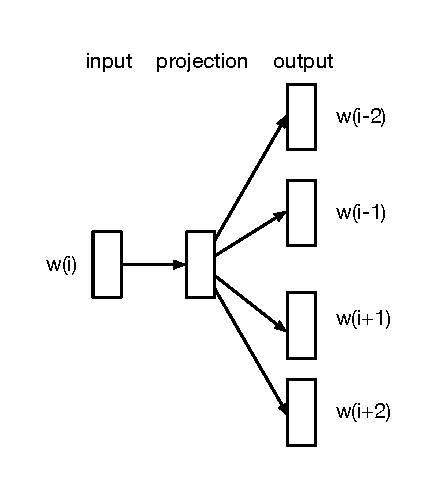
\includegraphics{./skip-gram.eps}
    \caption{word-level skip-gram}
    \label{fig:1a}
\end{subfigure}
\hfill
\begin{subfigure}[b]{0.55\textwidth}
    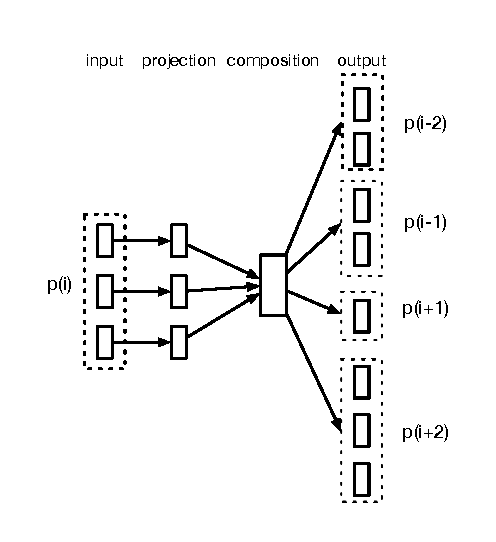
\includegraphics{./phrase-skipgram.eps}
    \caption{phrase-level skip-gram}
    \label{fig:1b}
\end{subfigure}
\caption{\small{Architecture of the skip-gram model.}}
\label{fig:skip-gram}
\vspace{-1em}
\end{figure}
The skip-gram model learns distributed vector representations for words by maximizing the probability of predicting
the context words given the current word. According to the \textit{word2vec} implementation of \namecite{mikolov2013distributed}, 
each input word $w$ is associated with a $d$-dimensional vector $v_w \in {\mathbb{R}}^{d}$ called the \textit{input embedding} and 
each context word $w_O$ is associated with a $d$-dimensional vector $v'_{w_O} \in {\mathbb{R}}^{d}$ called the \textit{output embedding}. $w, w_O$ are words from a vocabulary $V$
of size $W$. The probability of observing $w_O$ in the context of $w$ is modeled with a softmax function:
\begin{equation}
P(w_O | w) = \frac{\exp({v'_{w_O}}^T v_w)}{\sum_{i=1}^W \exp({v'_{w_i}}^T v_w)}
\end{equation}


The denominator of this function involves a summation over the whole vocabulary, which is impractical. One alternative 
to deal with the complexity issue is to sample several negative samples to avoid computing all the vocabulary. The objective
function after using negative sampling is:
\begin{equation}
    E_w = \sum_{w \in s} (\log \sigma ({v'_{w_O}}^T v_w) + \sum_{i=1}^{K} \log \sigma (-{v'_{w_i}}^T v_w))
\end{equation}
where $s$ is a chunked sentence. $w_i$, $i=1, 2, \ldots ,K$, are negative samples sampled from the following distribution:
\begin{equation}
P(w) = \frac{{\widetilde{P}(w)}^{\frac{3}{4}}}{Z}
\end{equation}
where $\widetilde{P}(w)$ is the unigram distribution of words and $Z$ is the normalization constant. The exponent $\frac{3}{4}$ is 
set empirically.
\section{Compositionality-aware skip-gram model}
\label{sec:compose}
To capture the way of composing phrase embeddings from distributed word vector representations, we extend the skip-gram model to include information from 
context of phrases and learn their compositionality from word vectors during the optimization procedure. Our phrase-level skip-gram structure is shown in
Figure~\ref{fig:1b}. 
\subsection{Phrase-level skip-gram model}
The word-level skip-gram model predicts the context words given the current word vector. Our approach further models the prediction of
context phrases given the vector representation of the current phrase vector (Figure~\ref{fig:1b}). Assume $v_p \in {\mathbb{R}}^d$ to be the $d$-dimensional 
input embedding for current phrase $p$ and $v'_{p_O}\in {\mathbb{R}}^d$ to be the output embedding for context phrase $p_O$. Using negative sampling, we model the phrase-level probability with:
\begin{equation}
\label{eq:phrase-skip}
    E_p = \sum_{p\in s} (\log \sigma ({v'_{p_O}}^T v_p) + \sum_{i=1}^{N} \log \sigma (-{v'_{p_i}}^T v_p))
\end{equation}
where $p_i$, $i= 1, 2, \ldots ,N$, are negative samples sampled according to the unigram probability of phrases raised to the same exponent $\frac{3}{4}$.


We jointly model word-level skip-gram and phrase-level skip-gram for each sentence:
\begin{equation}
E = E_w + \beta E_p
\end{equation}
where $\beta > 0$ adjusts the relative importance of the word-level and the phrase-level skipgram.
\subsection{Compositionality model}
Assume a phrase $p$ is composed of words $w_1, \ldots ,w_{n_p}$, where 
$n_p$ is the number of component words. The vector representation for $p$ is computed as:
\begin{equation}
    v_p = \Phi(\oplus( \sigma(v_{w_1}), \ldots ,\sigma(v_{w_i})))
\end{equation}
where $v_p$ is the vector representation for $p$. The function $\sigma$ is a component-wise manipulation over each dimension.
%, which can be intepreted as adjusting the dimensional values to the phrase vector space.
The symbol $\oplus$ is an operator over the component word vectors, which can be \textit{linear combination, summation, concatenation} etc. 
The mapping function $\Phi$ is a linear or non-linear manipulation over the resulting vector after the $\oplus$ operation. The same composition function is used to compute 
the output phrase embeddings $v'_{p_O}$ and $v'_{p_i}$, except that the component word vectors are $v'_{w_i}$ instead of $v_{w_i}$.


To show the effect of modeling phrase embeddings, we experiment with a composition function where $\oplus$ is \textit{linear combination} and $\Phi$ is passing the resulting matrix to the left of a weight vector $l^p = [l_1^p , l_2^p, \ldots, l_{n_p}^p]$
associated with each phrase $p$ showing how we combine the component word vectors. 
\begin{equation}
\label{eq:linear}
v_p = [\sigma(v_{w_1}), \ldots, \sigma(v_{w_{n_p}})] \begin{bmatrix} l_1^p \\ \vdots\\ l_{n_p}^p \end{bmatrix}
\end{equation}
where the function $\sigma$ is a component-wise power function over vector $v=[v_1, \ldots, v_n]$:
\begin{equation}
    \sigma(v) = [\phi(v_1), \ldots, \phi(v_n)]
\end{equation}
where $\phi(v_i)=\textit{sign}(v_i)|v_i|^{\alpha}$, $\alpha\geq 1$, is a power function over each dimension. This manipulation can be interpreted as adjusting dimensional values of word vectors to the phrase vector space.


Stochastic gradient ascent is used to update the word vectors. In equation~\ref{eq:phrase-skip}, for each word $w_j$ in $p'$, either context phrase $p_O$ or negative 
phrase sample $p_i$, the gradient is:
\begin{equation}
    \frac{\partial E_p}{\partial v'_{w_j}} = \triangledown \sigma(v'_{w_j}) (l_j^{p'} (y-\sigma({v'_{p'}}^T v_p)) v_p) 
\end{equation}
where $y=1$ for each word in $p_O$ and 0 for each word in $p_i$. $\triangledown \sigma(v'_{w_j})$ is a diagonal matrix where the $i$-th diagonal value is $\phi'({v'_{w_j}}_i)$.
For each word $w_j$ in the current phrase $p$, the gradient is:
\begin{equation}
\frac{\partial E_p}{\partial v_{w_j}} = \triangledown \sigma(v_{w_j}) (l_j^{p} ((1-\sigma({v'_{p_O}}^T v_p)) v'_{p_O} + \sum_{i=1}^{N} (-\sigma({v'_{p_i}}^T v_p)) v'_{p_i})) 
\end{equation}
\subsection{Output phrase embedding space}
Following \namecite{ling-EtAl:2015:NAACL-HLT} in 
using different output embeddings at each relative position to capture order information of context words (we call this \textit{positional} model), 
we use separate output embeddings to capture phrase-compositionality (we call this \textit{compositional} model). That is, we have a separate component 
word vector $v''$ to compose the phrase vectors in the context 
and the negative samples instead of using $v'$.
The intuition of this choice is that we don't want the compositionality information in the context or negative sample layer 
to be distorted by word-level updates. 


We further extend the phrase-level skipgram to include the order information, which
uses different output word embeddings to compose phrases at each relative position. Phrases at the same relative position share the same
output embeddings (we call this model \textit{positional+compositional}).
Without loss of generality, we experiment with the composition
described in Equation~\ref{eq:linear}. The coefficients $l_i^p$s are set to be $\frac{1}{n_p}$.
\section{Proposed methods}
\begin{table}
\centering
\begin{center}
\scalebox{0.75}{
\begin{tabular}{|l|l|l|l|l|l|l|} \hline
 length  & 1 & 2 & 3 & 4 & $\geq 5$\\ \hline
 frequency  & 525m & 137m & 62m & 22m & 15m\\ \hline
\end{tabular}}
\caption{\small{Statistics of phrase length distributions (m/million)}}
\label{tab:stats}
\end{center}
\end{table}
The phrases information are usually extracted using a chunker or based on pointwise mutual information (PMI).
For example, the phrases extracted using \textit{senna} suffer from the small average length for each phrase. We can see from 
Table~\ref{tab:stats} that most of the phrases are of length 1 and compositionality is used in very limited places.
Another problem with such kind of phrases is that the phrase boundaries are fixed and there is no way of learning compositionality
between two adjacent phrases, especially cases where different chunkings are all valid phrases. For example,
\textit{new zealand} and \textit{new zealand islanders} are both valid phrases, while \textit{senna} would chunk \textit{new zealand}
as a phrase and \textit{islanders} as a separate phrase.
\subsection{Joint MCMC sampling model}
MCMC algorithms have been used to extract phrases by iteratively going through the unlabeled data and sample from left to right, one variable at a time
at each sentence. Usually a nonparametric bayesian model based on a nonparametric prior, such as Dirichlet Process, is used to smooth the distribution of
the data and avoid overfitting. During the sampling procedure, the boundary variables would be sampled according to the posterior distribution and the phrases
in a sentence would vary whenever some of the boundary variables are flipped during the sampling procedure.


Therefore, we propose a joint MCMC sampling and compositionality learning model for phrase extraction and learning way of composing phrase embeddings. We use a log bi-linear
model to compute the probability of contexts given the phrase sequence:
\begin{equation}
P({\bf b},{\bf c}|{\bf w})= \frac{1}{Z}e^{\sum_i v'_{c_i} \cdot v_{p_i}}
\end{equation}
where ${\bf w}$ is the word sequence and ${\bf b}$ is the binary variable sequence which models the boundary information for each phrase in the sequence and ${\bf c}$ is the context sequence for the phrases in the sequence.
At each position $j$, we sample its binary value:
$$b_j \sim \frac{1}{Z} e^{\sum_i v'_{c_i} \cdot v_{p_i}}$$
where $Z$ is a constant which is agnostic to the value of $b_j$. In practice we don't have to compute all the terms in the summation as most of them are not affected by the choice $b_j$. The terms that needs to be recomputed
involves the phrases that are affected by $b_j$: $(p_1, p_2)$ when $b_j=1$ and $p_3$ when $b_j=0$. 


After we have sampled the boundary variable $b_j$ and whenever we have reached a new phrase, we use this new phrase to predict its context. This can be done using
the compositional skip-gram model we have introduced before and the vectors are updated during the procedure. As for the update, we consider a few choices for the time
of vector update: 1. whenever a binary variable is flipped. 2. whenever we have reached the end of a phrase (sampled a binary value 1). 3. update when the boundary for the whole sentence is decided.
\begin{algorithm}[t]
\small
\caption{A joint model for phrase extraction and compositionality learning}
\begin{algorithmic}[1]
\STATE{Initialize binary variables $b_1,\cdots, b_n$}
\FOR{$iter = 1,\cdots , T$:} 
    \FOR{$s = 1, \cdots, S$:}
        \FOR{$j = 1,\cdots , n$:}
            \STATE{Let $(p_1, p_2)$ be the two phrases when the $b_j=1$ and $p_3$ be the phrase when $b_j=0$}
            \STATE{Sample $b_j \sim \frac{1}{Z} e^{\sum_i v'_{c_i} \cdot v_{p_i}}$}
            \IF{$b_j = 1$}
                \STATE{Update $v_w$ for $w\in p_1$ according to the compositionality model}
            \ENDIF
        \ENDFOR
    \ENDFOR
\ENDFOR
\end{algorithmic}
\label{alg:joint}
\end{algorithm}
\subsection{Phrase independence variation}
In the previous section, we have modeled the probability of the whole sequence with a log bi-linear model. Here we consider factorizing the probability of the whole sequence into product of probility over individual phrases.
\begin{equation}
P({\bf b},{\bf c}|{\bf w}) = \prod_i P(c_i| p_i)
\end{equation}
where $P(c_i| p_i)$ is modeled with the standard skip-gram model.
\begin{equation}
P(c_i| p_i) = \prod_{p_j \in c_i} \frac{1}{Z} e^{v'_{p_j} v_{p_i}}
\end{equation}
where $Z$ is the normalization constant which sums over the whole phrase vocabulary $Q$.
\begin{equation}
Z = \sum_{p \in Q}e^{v'_p v_{p_i}}
\end{equation}
The summation over the whole vocabulary is impractical. One alternative is to use negative sampling which approximate the sum over the whole vocabulary with a few samples.
$$Z = \sum_{j} e^{v'_{p_j} v_{p_i}}$$
where $p_j$s are negative samples sampled from the same uniform distribution over phrases described in the previous sections.


We sample the binary value $b_j$ according to the following probabilities:
$$P(b_j = 1) \propto P(c_1 | p_1) \cdot P(c_2 | p_2) \cdot P(c')$$
$$P(b_j = 0) \propto P(c_3 | p_3)\cdot P(c")$$
where $P(c')$ and $P(c")$ evaluate the change of contexts for the surrounding phrases when the binary value varies.

\section{Future schedule}
I will first wrap up the compositional model learning without MCMC before the 2016 Fall. During 2016 Fall, I will partly work on using MCMC sampling to learn phrase boundaries for expand existing framework.
I will spend more time on this project after I have finished the previous two projects. Hopefully get this work done by the end of 2017 Spring. Possible target includes ACL 2017, IJCAI 2017 and EMNLP 2017.
\section{Conclusion}
In this section, we have introduced a joint model for learning phrase embeddings and phrase compositionality. To overcome the limits of the the short length of each phrase and to increase flexibility of 
phrase boundaries, we propose a joint model which uses an MCMC sampling schedule to learn flexible boundary of phrases and learns distributed phrase compositionality at the same time.

\break

%\chapter{Neural machine translation}
%\label{chap:nmt}
%Neural machine translation.

%\break
\chapter{Conclusion}
\label{chap:conclusion}
In this paper, I have proposed various applications of MCMC algorithms.
\break

\bibliographystyle{urcsbiblio}
\bibliography{long}
\appendix
\end{CJK}

\end{document}
